\documentclass[11pt,twoside,a4paper]{article}

\usepackage[pdftex]{graphicx}
\usepackage{setspace}
\usepackage{indentfirst}
\usepackage{listings}
\usepackage[utf8]{inputenc}
\usepackage[T1]{fontenc}
\usepackage{hyperref}
\usepackage{amssymb,amsmath}
\usepackage{algpseudocode,algorithm,algorithmicx}
\usepackage{xcolor}
\usepackage{float}
\lstset{basicstyle=\ttfamily,
  showstringspaces=false,
  commentstyle=\color{olive},
  keywordstyle=\color{blue}
}

\title{Machine Learning Engineer Nanodegree - Solving Breakout game with Deep Reinforcement Learning}
\author{Andr\'e Tadeu de Carvalho}
\date{\today}

\DeclareMathOperator*{\argmax}{argmax}

\begin{document}

\maketitle

\section*{I. Definition}

\subsection*{Project Overview}

Motivated by the growth of multi-player games market, the advent of esports, and
the rise of Deep Reinforcement Learning algorithms (DRL for brevity) to play
games with human-level performance, I will evaluate two Deep Reinforcement
Learning algorithms in this project against a classical Atari\texttrademark
game, \emph{Breakout}.

Deep Reinforcement Learning is a combination of reinforcement learning
approaches, that discovers how to perform a task by trial-and-error, and Deep
Learning, that approximates complex functions by using neural networks with
multiple layers of different kind.

\subsection*{Problem Statement}

For this project, I selected two DRL algorithms to evaluate in Breakout
environment. The DRL algorithms I chose to evaluate are:
\begin{enumerate}
  \item Deep-Q Learning algorithm, from Mnih et al\cite{mnih2015humanlevel}.
  \item A2C algorithm, from Mnih et al\cite{DBLP:journals/corr/MnihBMGLHSK16}.
\end{enumerate}

The objective of this project is to measure the algorithms performance in terms
of running time to converge, i.e. how many episodes are needed to the algorithm
to obtain good enough rewards or loss of Q-value, and the corresponding value
for each algorithm that indicates the algorithm, given its neural network
weights, can get better scores playing Breakout. This metrics will be further
explained later.

As stated in my Capstone proposal\cite{capstone-proposal}, Breakout is a game
which its objective is to destroy all of the bricks on the top of screen. To do
so, the player controls a paddle and use it to bounce a ball, which will bounce
back to the top of screen, hit the bricks, destroying them. The player wins
whenever all the bricks are destroyed and it loses whenever all the balls that
the player has available goes to the bottom of screen. I will use the
\emph{BreakoutNoFrameskip-v4} environment from OpenAI Gym\cite{openai-gym}
\cite{DBLP:journals/corr/abs-1207-4708} as the environment in which all the
learning agents will play.

The implementation of the algorithms are not mine. I ran the algorithms from
OpenAI baselines\cite{baselines} project, which I forked from OpenAI GitHub to make small
adaptations to automate the algorithm execution, available in
\url{https://github.com/andretadeu/baselines}. The source code is reliably
implemented in TensorFlow and I do not have to deal with code errors in
rounding numbers or incorrect use of Deep Learning APIs.

\subsection*{Metrics}

For this analysis, I am going to use the reward, the convergence time,
i.e how many hours are needed to the algorithm to return human-level performing
rewards and the corresponding Q-value or loss-value for each algorithm. These
are the performance metrics I am using because the scoreboard is the only
indicator the game provides to measure how well a player performs in a Breakout
game. The convergence time is used because I want to minimize the amount of time
needed to train an algorithm to play Breakout in human-level performance.

About how the metrics are obtained, the scoreboard is returned by OpenAI Gym
after each action and the convergence time is the time spent for the algorithm
to estabilize in some mean scores in a certain number of episodes. Since these
algorithms have a parameter to control the number of iterations, they might
converge before the number of iterations ends or they might oscilate and do not
show any vestige of convergence.

Regarding to the convergence time, running the experiments in the same machine
or AWS EC2 instance type, it indirectly addresses the amount of compute
resources used by the algorithm. Even though this proxy measure is imperfect for
this task, it is useful for the purpose of amount of money spent on AWS EC2
instances.

Even though the rewards come from the scoreboard and they is used to take an
action, each algorithm is a different proposition on how the rewards are used to
choose an action. The metrics below are used as supporting metrics,
to assist the examination whether the algorithms are learning to play Breakout
or they are failing to improve the performance measured, measured by the
scoreboard.

In the case of Deep-Q Learning algorithm, the reward and the future rewards are
taken into consideration, and a discount factor for the future rewards, taking
the timestep as exponent (from \cite{mnih2015humanlevel}):

$$
  Q*(s,a) = \max_{\pi}{\mathbb{E}\bigl[r_{t} + \gamma r_{t + 1} + \gamma^{2} r_{t + 2} + \ldots
  | s_{t} = s, a_{t} = a, \pi \bigr]}
$$

The current implementation for DQN algorithm already have the dueling
version to be set as parameter, which is \textbf{true} by default. Dueling DQNs
are presented in \cite{DBLP:journals/corr/WangFL15} and will be further
explained later. In terms of metrics, the algorithm optimizes the function

$$
  Q(s,a;\boldsymbol{\theta},\alpha,\beta) =
  V(s;\boldsymbol{\theta},\beta) + \biggl( A(s,a;\boldsymbol{\theta},\alpha)
  - \frac{1}{|\mathcal{A}|} \sum_{a'} A(s,a';\boldsymbol{\theta},\alpha) \biggl),
$$

\noindent according to the OpenAI implementation of dueling DQNs model. Here,
$ \boldsymbol{\theta} $ is the convolutional layers parameters and $ \alpha $
and $ \beta $ are the weights of the fully connected layers.

A2C algorithms estimates the advantage of taking an action
$ a_{t} $ given the learner is in state $ s_{t} $, by subtracting the
estimated value for $ V^{\pi}(s_{t}) $ from the estimated value of
$ Q^{\pi}(s_{t},a_{t}) $, or $ A(s_{t},a_{t}) = Q(s_{t},a_{t]}) - V(s_{t}) $
\cite{DBLP:journals/corr/MnihBMGLHSK16}, or variations of the actor-critic
architecture, also described in \cite{DBLP:conf/amcc/DegrisPS12}.
The actor-critic architecture will be properly explained in Algorithms section.

The results of these metrics will show whether the algorithm is converging to
a human-level performance agents in Breakout or these actors are troubling to
learn to play the game.

\section*{II. Analysis}

\subsection*{Environment Exploration}

The environment is the game BreakoutNoFrameskip-v4, from Atari 2600, with 210
pixels x 160 pixels x 3 channels of color, 128 colors supported by Atari. The
game consists of a paddle on the bottom of the screen, a bouncing ball, and
layers of bricks on the top of the screen.

\begin{figure}[H]
  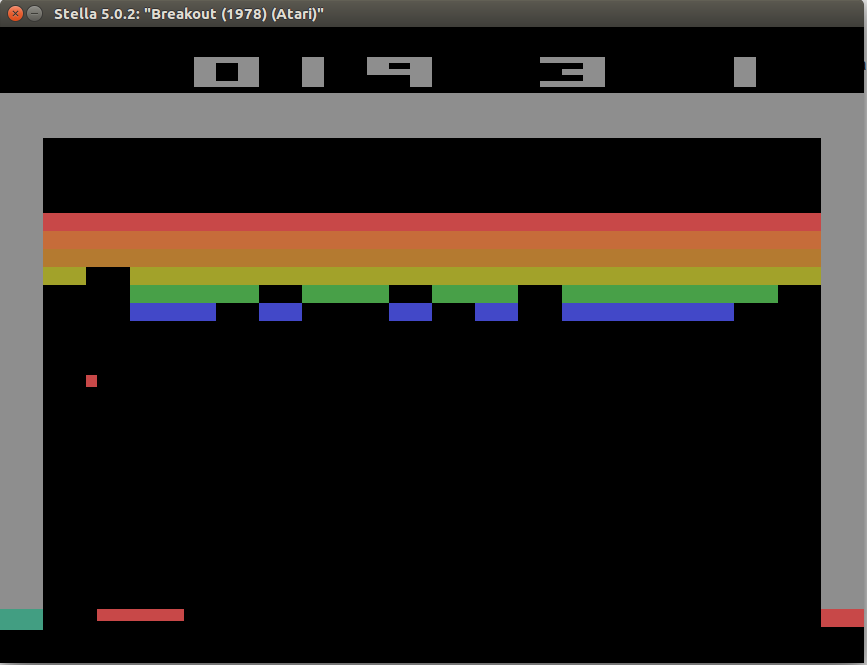
\includegraphics[scale=0.25]{images/breakout-01.png}
  \centering
  \caption{Atari 2600 Breakout game in Stella}
  \label{fig:breakout-01}
\end{figure}

In addition, the game has the number of lives and the scoreboard. The number of
lives is only useful to when reaches zero, which is the end of game. The
scoreboard is where the learning agent obtain its rewards and evaluate it with
one of the algorithms to calculate a value to choose the next action.
Furthermore, Atari games also emits sounds, which are not useful to solve this
problem.

\subsection*{Algorithm and Techniques}

Since I am evaluating two algorithms, I will provide a simple explanation
about the algorithms, and describe all the parameters used. Before that, a
simple explanation about Deep Reinforcement Learning is needed.

Deep Reinforcement Learning is an approach to use deep neural networks to
calculate a complex function which results in choosing an action or receiving a
certain reward. After that, the traditional part of Reinforcement Learning is
evaluated, whether the policy results in an action, or a Q-value is calculate,
or even it is an actor-critic algorithm, requiring to calculate an advantage
function.

Only relying on the current experience of the training seems to be not enough.
To be effective, Deep Reinforcement Learning requires to store all the
experiences and randomly sampling them to use during training.

\begin{figure}[h!]
  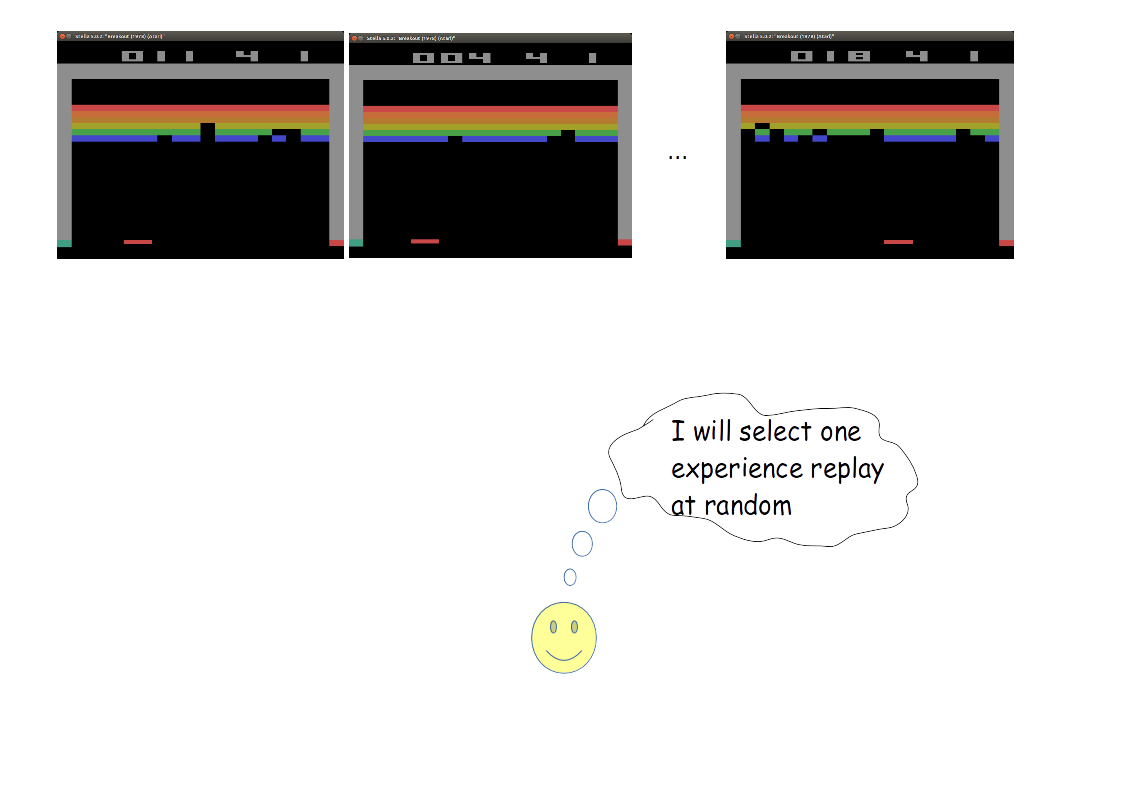
\includegraphics[width=\linewidth]{images/ExperienceReplay.png}
  \caption{Deep neural network from DQN}
  \label{fig:experience-replay}
\end{figure}

By using the experience, it is possible to improve over them and generate even
better experiences to improve upon. Experience replay is used in all the
algorithms presented below. Now it is time to describe them.

These two algorithms requires the use of Convolutional layers, as
documented in \emph{Human-level control through deep reinforcement learning}
\cite{mnih2015humanlevel}. Convolutional layers are neural network layers where
the outputs are obtained by sliding a kernel window with some weights into the
input tensor and obtaining an output, which might be smaller than the input.

A convolutional layer constitutes of the following parameters:

\begin{itemize}
  \item Input size - $ x = \rm I\!N^n $ where $ n > 0 $ is the number of the input dimensions.
  It is the input where the convolution will be performed.
  \item Kernel size - $ k = \rm I\!N^n $ where $ n > 0 $ is the number of the input dimensions.
  It is the kernel filter with all the weights to compute the convolution.
  \item Stride - How much the window will slide. Generally is a $ k = \rm I\!N > 0 $ value.
  \item Padding - How many layers and columns with zeroes will be concatenaded with the input data.
\end{itemize}

Here is one example below:

\begin{figure}[h!]
  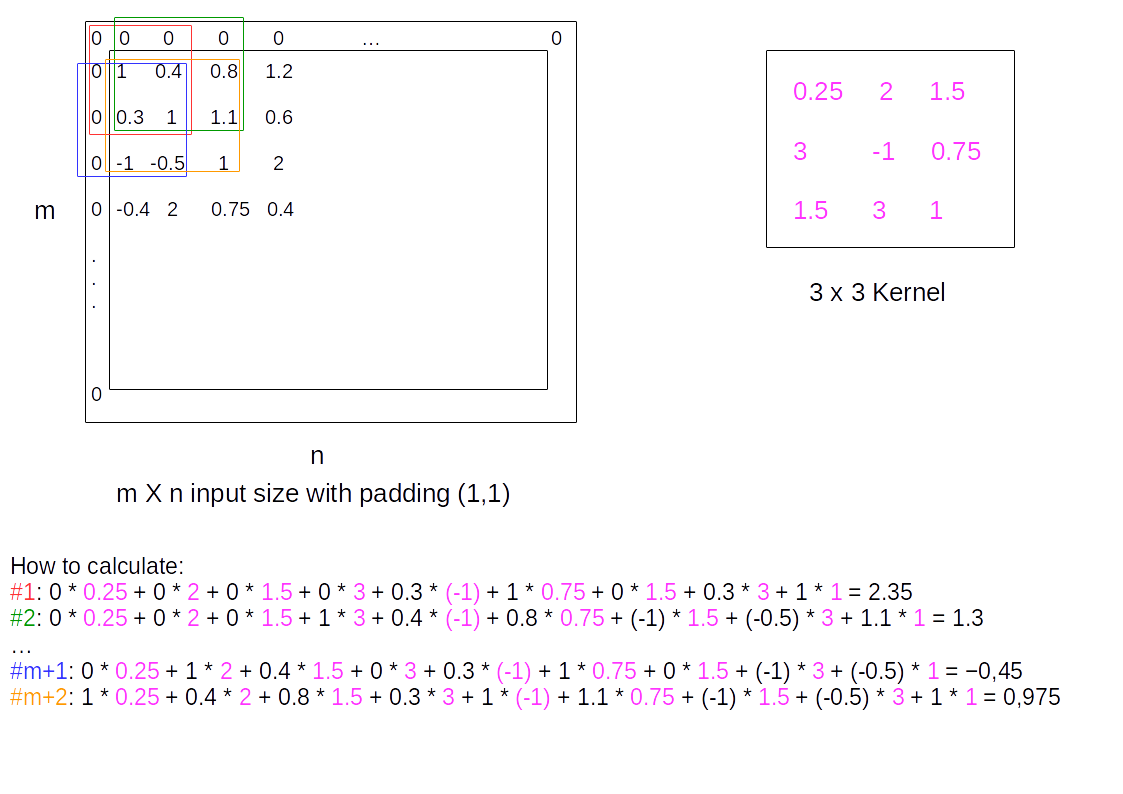
\includegraphics[width=\linewidth]{images/CNN-example.png}
  \caption{Example of a CNN with dimensions m X n}
  \label{fig:cnn-example}
\end{figure}

In this example, the input is a matrix $ A $ with sizes $ m \times n $, the
kernel is a $ 3 \times 3 $ matrix, the padding is 1 for width and height, and
the stride is 1. The output matrix $ B $ is of dimensions:

$$
B_{x} = \frac{A_{x} - k_{x} + 2p_{x}}{S}
$$

In this example, if $ m = n = 32 $, the dimensions of $ B $ is:

$$
B_{x} = B_{y} = \frac{32 - 3 + 2 \cdot 1}{1} = 31
$$

In addition, both algorithms use ReLU functions, which are incredibly simple and
powerful. ReLU functions are functions where equals and below zero, the output
of the function is zero, and above zero the function is linear.

$$
f(x) =
\begin{cases}
  0 & if x \leq 0 \\
  x & otherwise
\end{cases}
$$

or, more succintly $ f(x) = max(0, x) $.

\subsubsection*{Deep Q-Learning}

An implementation with several features was provided by OpenAI, which enables
the user to choose whether to use one technique or the other. At the same time
I will explain how the algorithm works, implemented in the archive
\textit{baselines/deepq/models.py}, I will give a brief
presentation of the techniques employed.

The reduced input comes from atari-py and it is returned from OpenAI Gym
\textbf{env} variable, and it evaluated using the deep neural network
architecture described in the next figure.

\begin{figure}[h!]
  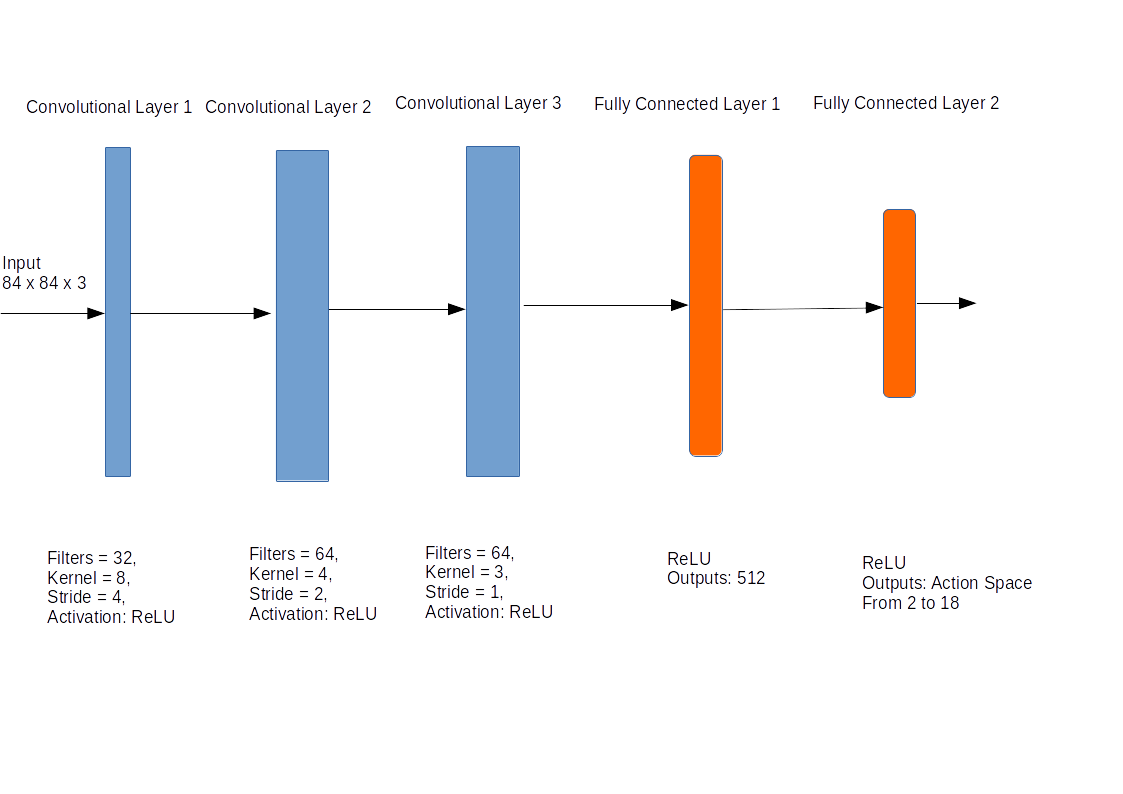
\includegraphics[width=\linewidth]{images/DQN-architecture.png}
  \caption{Deep neural network from DQN}
  \label{fig:dqn-architecture}
\end{figure}

Both the data and the target are evaluated against this network. After that,
the algorithm calculate the Q-scores from the actions that the algorithm
selected. After that, it is calculated the Q-score for the best action returned
by the algorithm. Now, we have everything to calculate the Bellman equation:

$$ Q(s_{t},a_{t}) = r + \gamma \cdot Q(s_{t + 1},a_{t + 1}) $$

Once we calculated the Bellman equation, we need to calculate the error, by
using a loss function, which in this implementation of the algorithm is the
Huber Loss\cite{huber_loss}, and use the importance weights to get a weighted
error.

$$
L_{\delta}(y,f(x)) =
\begin{cases}
  \frac{1}{2}(y - f(x))^2 & for \left|y - f(x)\right| \leq \delta,\\
  \delta\left|y - f(x)\right| - \frac{1}{2}\delta^2 & otherwise.
\end{cases}
$$

Once the weighted error is calculated, it is possible to calculate the gradient
to obtain the amount to update and follow the gradient. In my experiment, I did
not clip the gradients.

There is an option to create perturbations in the parameter space as described
in \cite{DBLP:journals/corr/PlappertHDSCCAA17}, calculating some random values
from Ornestein-Uhlenbeck process and adding this values in the parameter space.
I have this parameter set as \textbf{false} by default in the
\textit{baselines/deepq/experiments/run\_atari.py}.

In addition, I let the parameter for Double Deep Q-Learning
\cite{DBLP:journals/corr/HasseltGS15}, which solve the issue of DQN overshooting
the parameters $ \boldsymbol{\theta} $. According to this article, decomposing
the \textbf{max} operation from action selection and action evaluation really
reduces the value estimation and improve scores by obtaining a new
$ \boldsymbol{\theta}^{-}_{t} $ evaluating the deep neural network with the
target parameter $ \boldsymbol{\theta}'_{t} $ returned from the previous common
step of target Q-value evaluation and replacing the target parameter
$ \boldsymbol{\theta}'_{t} $ with $ \boldsymbol{\theta}^{-}_{t} $:

$$
Y^{DoubleDQN}_{t} \equiv R_{t + 1} +
\gamma Q(S_{t + 1},\argmax_{a} Q(S_{t + 1},a;\boldsymbol{\theta}_{t}),\boldsymbol{\theta}^{-}_{t}).
\cite{DBLP:journals/corr/HasseltGS15}
$$

Other improvement over standard DQN algorithms I am using is the Dueling DQN.
Basically separating the calculating the value function from Deep Q-Network and
an advantage function. The equation presented in metrics will suffice, but this
approach also reflects in the deep neural network architecture, which is
presented below.

\begin{figure}[h!]
  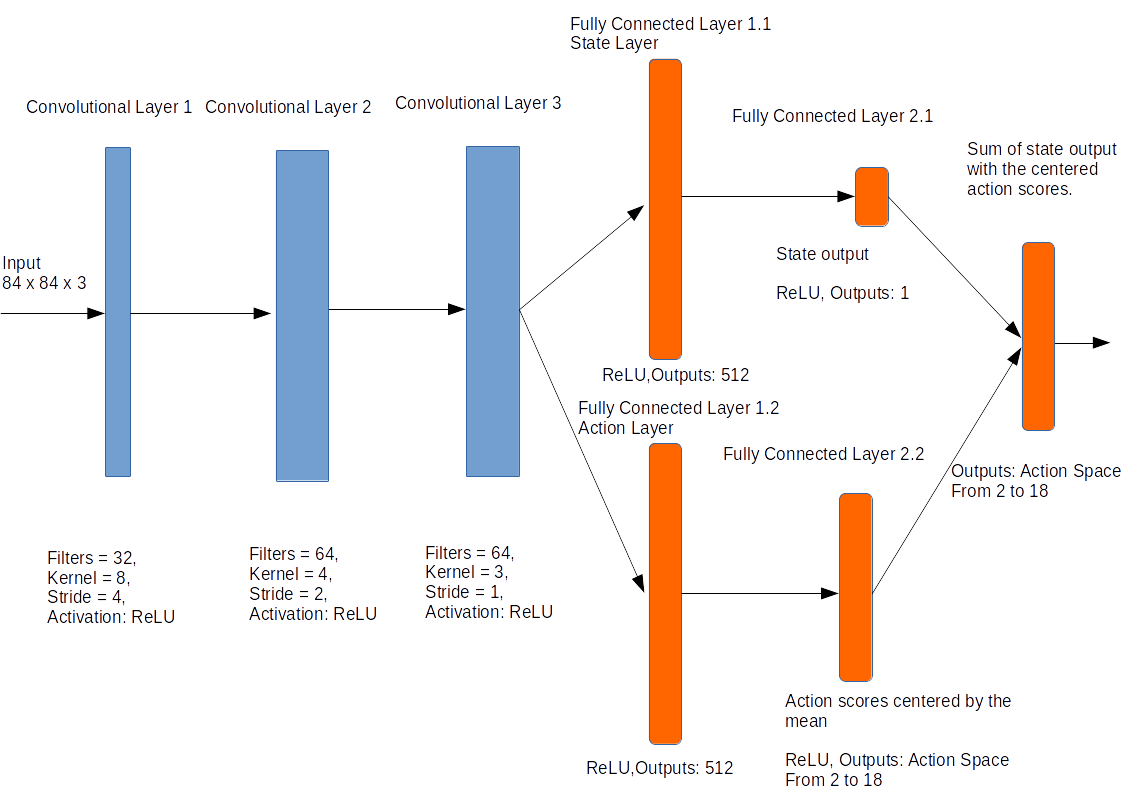
\includegraphics[width=\linewidth]{images/Dueling-DQN-architecture.png}
  \caption{Deep neural network from Dueling-DQN}
  \label{fig:dueling-dqn-architecture}
\end{figure}

The last improvement comes from prioritized replays
\cite{DBLP:journals/corr/SchaulQAS15}. The authors of this article propose a
prioritized way to choose the experience replays according to its
\emph{Temporal-Difference error}, from the highest to the lowest. The experiences
with high TD errors are the ones that makes the agent learn more efficiently.
Another property of the prioritized replays are to distinguish which transitions
are interesting to keep and the ones that can be discarded, saving memory.

Finally, the parameters recommended by OpenAI:

\begin{center}
  \begin{tabular}{ | l | c | r | }
    \hline
    \textbf{Learning Rate} & 0.0001 \\ \hline
    \textbf{Number of Timesteps} & 1,000,000 \\ \hline
    \textbf{Buffer size} & 10,000 \\ \hline
    \textbf{Fraction of training period for exploration} & 0.1 \\ \hline
    \textbf{Final exploration factor} $ \boldsymbol{\epsilon} $ & 0.01 \\ \hline
    \textbf{Training Frequency} & 1 \\ \hline
    \textbf{Batch size} & 32 \\ \hline
    \textbf{Print out frequency} & 100 steps \\ \hline
    \textbf{Checkpoint frequency} & 10,000 steps \\ \hline
    \textbf{Timestep where learning starts} & 10,000th timestep \\ \hline
    \textbf{Discount factor} $ \boldsymbol{\gamma} $ & 0.99 \\ \hline
    \textbf{Target network update frequency} & 500 \\ \hline
    \textbf{Prioritized Replay} & true \\ \hline
    \textbf{Prioritized Replay} $ \boldsymbol{\alpha} $ & 0.4 \\ \hline
    \textbf{Prioritized Replay} $ \boldsymbol{\beta} $ & 0.6 \\ \hline
    \textbf{Number of iterations} $ \boldsymbol{\beta} $ \textbf{will be annealed} & 1,000,00 \\ \hline
    \textbf{Prioritized Replay} $ \boldsymbol{\epsilon} $ & 0.000001 \\ \hline
    \textbf{Parameter Noise} & false \\
    \hline
  \end{tabular}
\end{center}

\subsubsection*{A2C}

In the article 'Asynchronous Methods for Deep Reinforcement Learning'
\cite{DBLP:journals/corr/MnihBMGLHSK16}, the authors use parallel actor-learners
in four Reinforcement Learning algorithms. These actor-learners are employed to
calculate and update the gradient descent asynchronously.

Instead of dealing with prioritized replays, this algorithm relies on several
learners and do not use any sort of prioritized replays. The A2C algorithm
relies on synchronization to update de parameter $ \boldsymbol{\theta} $ of the
neural network. After n-steps, the gradients update of each thread is used
to update $ \boldsymbol{\theta} $ synchronously (dropping one 'A' from A3C).

As an Actor-Critic method, the algorithm must evaluate the policy and the value,
using the value-based part of the algorithm to improve the policy. Given
$ \boldsymbol{\theta} $ as the parameters for the policy and
$ \boldsymbol{\theta}_{\upsilon} $ as the parameter for the value function, $T$
for the globally shared number of timesteps, $ t $ for thread step counter, the
algorithm is described below, adapted from \cite{DBLP:journals/corr/MnihBMGLHSK16}

\newpage

\begin{algorithm}
  \caption{Synchronous Advantage Actor-Critic learner \label{alg:a2c-thread}}
  \begin{algorithmic}[1]
    \State $ t \leftarrow 0 $
    \State // This repeat below is executed synchronously in N-threads
    \Repeat
      \State // Reset the gradients
      \State $ \textbf{d}\boldsymbol{\theta} \leftarrow \vec{0} $
      \State $ \textbf{d}\boldsymbol{\theta}_{\upsilon} \leftarrow \vec{0} $
      \State // Synchronize thread specific Parameters
      \State $ \boldsymbol{\theta}' \leftarrow \boldsymbol{\theta} $
      \State $ \boldsymbol{\theta}'_{\upsilon} \leftarrow \boldsymbol{\theta}_{\upsilon} $
      \State $ t_{start} \leftarrow t $
      \State Get state $ s_{t} $
      \Repeat
        \State Perform $ a_{t} $ according to policy $ \pi(a_{t}|s_{t};\boldsymbol{\theta}) $
        \State Receive reward $ r_{t} $ and new state $ s_{t + 1} $
        \State $ t \leftarrow t + 1 $
        \State $ T \leftarrow T + 1 $
      \Until{terminal $ s_{t} $ or $ t - t_{start} == t_{max} $}
      \If{$ s_{t} $ is terminal}
        \State $ R \leftarrow 0 $
      \Else
        \State $ R \leftarrow V(s_{t},\boldsymbol{\theta}'_{\upsilon}) $
      \EndIf
      \For{$ i \in \{t - 1, \ldots, t_{start}\} $}
        \State $ R \leftarrow r_{i} + \gamma R $

        \State $ \textbf{d}\boldsymbol{\theta} \leftarrow \textbf{d}\boldsymbol{\theta}
        + \nabla_{\boldsymbol{\theta}'} \log{\pi(a_{i}|s_{i};\boldsymbol{\theta}')(R - V(s_{i};\boldsymbol{\theta}'_{\upsilon}))} $

        \State $ \textbf{d}\boldsymbol{\theta}_{\upsilon} \leftarrow \textbf{d}\boldsymbol{\theta}_{\upsilon}
        + \frac{\partial (R - V(s_{i};\boldsymbol{\theta}'_{\upsilon}))^{2}}{\partial \boldsymbol{\theta}'_{\upsilon}}$
      \EndFor
      \State Update $ \boldsymbol{\theta} $ synchronously by aggregating all $ \textbf{d}\boldsymbol{\theta} $
      \State Update $ \boldsymbol{\theta}_{\upsilon} $  synchronously by aggregating all $ \textbf{d}\boldsymbol{\theta}_{\upsilon} $
    \Until{$ T > T_{max} $}
  \end{algorithmic}
\end{algorithm}

I ran the algorithm with the standard version of the A2C algorithm, that uses
CNNs as function approximators, which is the same function approximator from the
DQN algorithm. There are other implemented functions, such as Log-LSTM, LSTM and
MLP, but I decided to use the defaults.

Another implementation consideration is that this implementation uses RMSProp
optimizer, so we need a decay parameter $ \alpha $. The intuition behind RMSProp
is to avoid overshooting in the updates, so it divides the learning rate with
the Root Mean Square of the gradient to update weight parameters of the neural
network. First, we need to calculate $ \upsilon(\alpha,t) $:

$$
\upsilon(\alpha,t) \leftarrow \alpha \cdot \upsilon(\alpha,t - 1) + (1 - \alpha) \cdot (\nabla J_{i}(w))^{2}
$$

where $ \alpha $ is the forgetting factor, $ t $ is the timestep, $ \nabla J_{i}(w) $
is the gradient of the loss function, and $ w $ are the weight parameters of the
neural network.

After that, the weights can be update:

$$
w_{t + 1} \leftarrow w_{t} - \frac{\eta}{\sqrt{\upsilon(\alpha,t)}}\nabla J_{i}(w)
$$

Further details in \cite{rmsprop}\cite{rmsprop-coursera}.

Finally the parameters recommended by OpenAI:

\begin{center}
  \begin{tabular}{ | l | c | r | }
    \hline
    \textbf{Policy Model} & CNN \\ \hline
    \textbf{Number of steps} & 5 \\ \hline
    \textbf{Total timesteps} & 80,000,000 \\ \hline
    \textbf{Value-function coefficient} & 0.5 \\ \hline
    \textbf{Entropy coefficient} & 0.01 \\ \hline
    \textbf{Maximum gradient norm (Gradient clipping)} & 0.5 \\ \hline
    \textbf{Learning Rate} & 0.0007 \\ \hline
    \textbf{Exploration Factor} $ \boldsymbol{\epsilon} $ & 0.00005 \\ \hline
    \textbf{Forgetting Factor for RMSProp} $ \boldsymbol{\alpha} $ & 0.99 \\ \hline
    \textbf{Discount Factor} $ \boldsymbol{\gamma} $ & 0.99 \\ \hline
    \textbf{Log interval} & 100 timesteps \\ \hline
    \textbf{Learning Rate Schedule} & Constant \\
    \hline
  \end{tabular}
\end{center}

For an intuitive explanation of A2C algorithm, I recommend the following blog
post \url{https://hackernoon.com/intuitive-rl-intro-to-advantage-actor-critic-a2c-4ff545978752}
\cite{intuitive_a2c}.

\subsection*{Benchmark}

For benchmark, I am using the average of best human scores from
\url{http://www.jvgs.net/2600/top50.htm} and I am comparing them to the average
scores returned by the algorithms. Since the metrics returned are summed scores
and the number of rollouts for each episode, this way to compare human
perfomance versus algorithms' performance is fair.

From the link in the paragraph above, the scores are:

\begin{center}
  \begin{tabular}{ | l | c | r | }
    \hline
    \textbf{Ranking} & \textbf{Score} \\ \hline
    \textbf{\#1} & 864 \\ \hline
    \textbf{\#2} & 825 \\ \hline
    \textbf{\#3} & 812 \\ \hline
    \textbf{\#4} & 667 \\ \hline
    \textbf{\#5} & 532 \\ \hline
    \textbf{\#6} & 456 \\ \hline
    \textbf{\#7} & 424 \\ \hline
    \textbf{\#8} & 420 \\ \hline
    \textbf{\#9} & 408 \\ \hline
    \textbf{\#10} & 401 \\
    \hline
  \end{tabular}
\end{center}

\begin{itemize}
  \item Mean score: 580.9
  \item Median score: 494
\end{itemize}

I believe these score are better metrics than the baseline reported in DQN
DeepMind's article\cite{mnih2015humanlevel}, which is 31.8 (in average).

For curiosity, my top score playing in Stella emulator for Linux is 360.

\begin{figure}[H]
  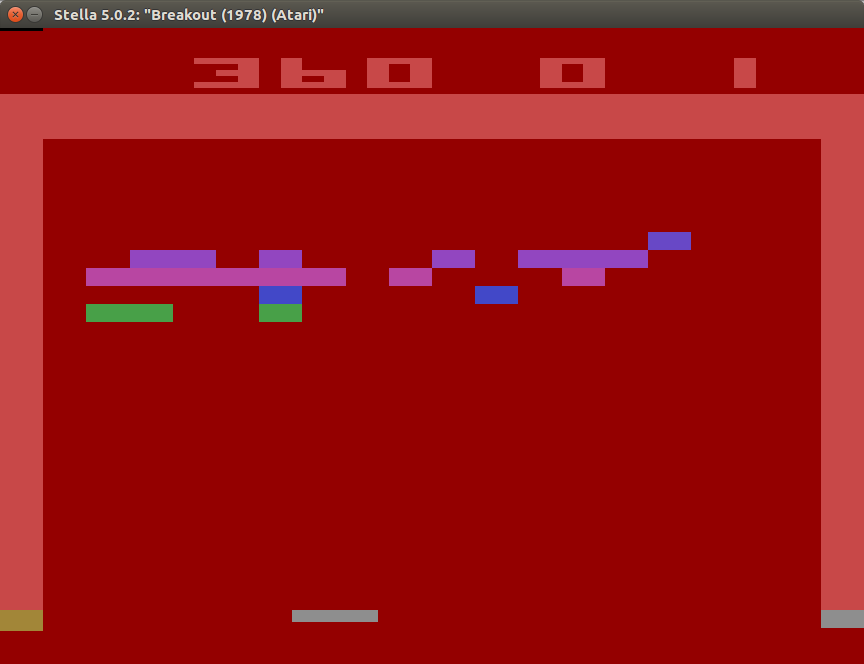
\includegraphics[scale=0.25]{images/top-score.png}
  \centering
  \caption{Author's top score}
  \label{fig:top-score}
\end{figure}

\subsubsection*{Why I chose these algorithms}

The algorithms were chosen because these are the simplest ones among Deep
Reinforcement Learning algorithms and are reasonable candidates for being used
as baseline algorithms (being in OpenAI baselines project explains a lot).

\subsection*{How to reproduce}

To compare the algorithms, I needed to create an Amazon AMI as a reference on
what I should have to have installed in my laboratory virtual machine. I used
the Deep Learning AMI 2.0 (\emph{ami-3b6bce43}) from Amazon as reference and
enriched it with:

\begin{itemize}
  \item OpenAI gym (All the packages),
  \item HDF5,
  \item h5py,
  \item cloudpickle,
  \item swig,
  \item language-pack-pt,
  \item OpenCV,
\end{itemize}

generating the image \emph{ami-1c79d264}. In addition, in this image I have
created a shell script to help to run all the experiments without having to wait
every one of them to finish. Furthermore I edited the file \emph{.bashrc} to
set \emph{OPENAI\_LOGDIR} and \emph{OPENAI\_LOG\_FORMAT} and to load the
python virtualenv for TensorFlow with Python 3.6.

Inside the folder \textit{/home/ubuntu/workspace/baselines}, the shell script
to run the experiments, \textit{capstone-analysis.sh}, contains:

\begin{lstlisting}[language=bash,caption={bash version}]
#!/bin/bash

source activate tensorflow_p36

export OPENAI_LOGDIR=${OPENAI_LOGDIR:-"${HOME}/openai-logs"}
export OPENAI_LOG_FORMAT=${OPENAI_LOG_FORMAT:-"tensorboard,csv"}

echo "== Start of experiments =="

# time python -m baselines.deepq.experiments.run_atari \
# --log-dir=${OPENAI_LOGDIR}/deepq/atari" \
# --log-formats="${OPENAI_LOG_FORMAT}"
time python -m baselines.a2c.run_atari \
--log-dir="${OPENAI_LOGDIR}/a2c/atari" \
--log-formats="${OPENAI_LOG_FORMAT}"
time python -m baselines.acer.run_atari \
--log-dir="${OPENAI_LOGDIR}/acer/atari" \
--log-formats="${OPENAI_LOG_FORMAT}"

echo "== End of experiments =="
\end{lstlisting}

I commented out the execution of DQN algorithm because it takes around 21 hours
to complete the whole training, which takes only around 2 hours for A2C
algorithm. The results of the algorithms are in CSV, provided by OpenAI
baselines, and HDF5 formats used by TensorBoard. The results will be explained
in 'Results' section.

In a new version of this image, the AMI \emph{ami-f9046981}, I redone the
experiments with the standard parameters and some variations to confirm that
OpenAI recommended parameters are, in fact, the best parameters. The shell
script \textit{capstone-analysis.sh} was modified as below:

\begin{lstlisting}[language=bash,caption={bash version}]
#!/bin/bash

source activate tensorflow_p36

export OPENAI_LOGDIR=${OPENAI_LOGDIR:-"${HOME}/openai-logs"}
export OPENAI_LOG_FORMAT=${OPENAI_LOG_FORMAT:-"tensorboard,csv"}

echo "== Start of experiments =="

time python -m baselines.deepq.experiments.run_atari \
--log-dir="${OPENAI_LOGDIR}/deepq/atari/0" \
--log-formats="${OPENAI_LOG_FORMAT}"
time python -m baselines.a2c.run_atari \
--log-dir="${OPENAI_LOGDIR}/a2c/atari/0" \
--log-formats="${OPENAI_LOG_FORMAT}"
time python -m baselines.deepq.experiments.run_atari \
--log-dir="${OPENAI_LOGDIR}/deepq/atari/1" \
--log-formats="${OPENAI_LOG_FORMAT}" --dueling=0
time python -m baselines.a2c.run_atari \
--log-dir="${OPENAI_LOGDIR}/a2c/atari/1" \
--log-formats="${OPENAI_LOG_FORMAT}" --lrschedule=linear
time python -m baselines.a2c.run_atari \
--log-dir="${OPENAI_LOGDIR}/a2c/atari/2" \
--log-formats="${OPENAI_LOG_FORMAT}" --policy=lstm
time python -m baselines.a2c.run_atari \
--log-dir="${OPENAI_LOGDIR}/a2c/atari/3" \
--log-formats="${OPENAI_LOG_FORMAT}" \
--lrschedule=linear --policy=lstm
time python -m baselines.a2c.run_atari \
--log-dir="${OPENAI_LOGDIR}/a2c/atari/4" \
--log-formats="${OPENAI_LOG_FORMAT}" --policy=lnlstm
time python -m baselines.a2c.run_atari \
--log-dir="${OPENAI_LOGDIR}/a2c/atari/5" \
--log-formats="${OPENAI_LOG_FORMAT}" \
--lrschedule=linear --policy=lnlstm

echo "== End of experiments =="
\end{lstlisting}

\section*{III. Methodology}

\subsection*{Data processing}

Due to the input size, the colors of the input are going to be compressed to
reduce the state size and the images are rescaled to 84 x 84 pixels. The sounds
of the game are irrelevant for this problem and is not in the input. All these
approaches came from the Nature article about DQN\cite{mnih2015humanlevel} in
Methods section.

OpenAI implementation already has all these input compressions implemented in
\textit{baselines/common/atari\_wrappers.py} and it is used in all their
learners.

Besides compressing the input from Atari emulator, no further data processing
is done.

\subsection*{Implementation}

I chose those algorithms implementations because they were verified by
specialists about its correctness, these algorithms are relatively simple,
compared to other state-of-art algorithms (which means quite the opposite in
absolute terms), they are good as introductory algorithms to Deep
Reinforcement Learning, and these algorithms are close to state of art in terms
of technical knowledge involved.

Since these implementations are not mine, I am not forced to explain the code. I
will do it with the undocumented parts. All the documentation that is absent in
the code I intend to place in this report.

\subsubsection*{DQN details}

DQN implementation provided by OpenAI is a full-featured version one, which
increases substantially the knowledge level required to read the code and it is
a barrier for non-specialists.

As in other implementations, all begins in \textit{run\_atari.py} file, in this
implementations is located in \textit{baselines/deepq/experiments}. The model
used in DQN is obtained in this file, in line 24. The file
\textit{baselines/deepq/models.py} contains the function \textit{cnn\_to\_mlp},
which creates a TensorFlow model for a CNN and generates a MLP from it, which
is effectively done in line 33 of \textit{models.py}, in the function
\textit{\_cnn\_to\_mlp}. The \textbf{conv} parameter is a list of tuples with 3
elements. The format is:

(Number of outputs, kernel size, stride).

Iterating over these tuples from the parameter, this function create all the
convolutional layers in a generic way, but all using ReLU.

From line 44-51, in
\textit{action\_value} variable scope, the fully-connected layers from the
model are created, with or without normalization, depending on
\textbf{layer\_norm} boolean parameter. In the remaining lines of this method,
the dueling layers are created if the variable \textbf{dueling} is set. It also
depends on whether the layer should be normalized or not. More details about
TensorFlow variable scope is in
\url{https://www.tensorflow.org/api_docs/python/tf/variable_scope}.

The other files, functions, and classes are well documented and they need not be
explained further.

\subsubsection*{A2C details}

This A2C implementation is a complete one from the article. It allows to set
the architecture of the neural network for the policy, from a CNN, a LSTM, a
LNLSTM, and a MLP. All but the MLP architecture use the CNN part of the Nature
\cite{mnih2015humanlevel} paper.

LSTM policy used the CNN part and add LSTM layers. The number of layers is the
number of steps, or \textbf{nsteps}. To read this in the code, the sequential
elements returned from \textit{batch\_to\_seq}, in file
\textit{baselines/a2c/policies.py} are in lines 71 and 72 for LSTM. This
function reshapes the input data to a matrix of dimensions $ M_{(nbatch,nsteps)} $
and it splits in subtensors of \textbf{nbatch} size. The LSTM layer itself is
a vanilla one.

LNLSTM is a layer normalization technique introduced in \cite{LayerNorm}.
Except for layer normalization, LNLSTM follows the same implementation of LSTM
policy.

The model definitions are in \textit{baselines/a2c/a2c.py}. It defines all the
computations the model performs besides the policy. The Runner class contains
the \textbf{run} method, that, as it name says, runs the model, execute the
\textbf{step} method, and calculates the discounted reward. The learning
algorithm runs in batches, so in function \textbf{learn} in \textit{a2c.py}
divides the total of timesteps with the batch size, or \textbf{nbatch}. The
algorithm calculates \textbf{nbatch} as follows:

$$
nbatch = nenv \times nsteps
$$

where \textbf{nenv} is the number of environments and \textbf{nsteps} is the
number of steps, which the default value is 5.

\subsection*{Evaluated parameters}

For these experiments, I setup some parameters OpenAI baselines made available
to be changed. In DQN algorithm, I set the parameter \textbf{dueling} to false
in one separate execution. In A2C, I executed the algorithm with different
architectures and different learning schedules.

Here are the A2C executions with the following parameters:

\begin{center}
  \begin{tabular}{ | l | c | r | }
    \hline
    \textbf{Execution Number} & \textbf{Policy Model} & \textbf{Learning Rate Schedule} \\ \hline
    \#1 & cnn & constant \\ \hline
    \#2 & cnn & linear \\ \hline
    \#3 & lstm & constant \\ \hline
    \#4 & lstm & linear \\ \hline
    \#5 & lnlstm & constant \\ \hline
    \#6 & lnlstm & linear \\
    \hline
  \end{tabular}
\end{center}

The remaining parameters were left alone, using the recommended values.

\section*{IV. Results}

After almost a day of data processing, the results show that the DQN algorithm
takes 21 hours and 16 minutes to have less than the best human-level
performance. It achieves a summed reward around 230, in a mean of 100 episodes.
In contrast, A2C algorthm takes only 2 hours and 16 minutes and get better
scores than DQN, in average. It obtains a summed reward around 350, averaged
between all actors that executed the episode. Some actors took more episodes to
finish and some took less episodes.

To get a sense how the algorithms are performing, I extracted the graphs
generated by TensorBoard and I generated the graphs from the data in CSV. The R
script I use to generate the graphs are in \emph{log-analysis} folder.

\subsection*{DQN}

From the TensorBoard data, the results I obtained from the first experiment:

\begin{figure}[H]
  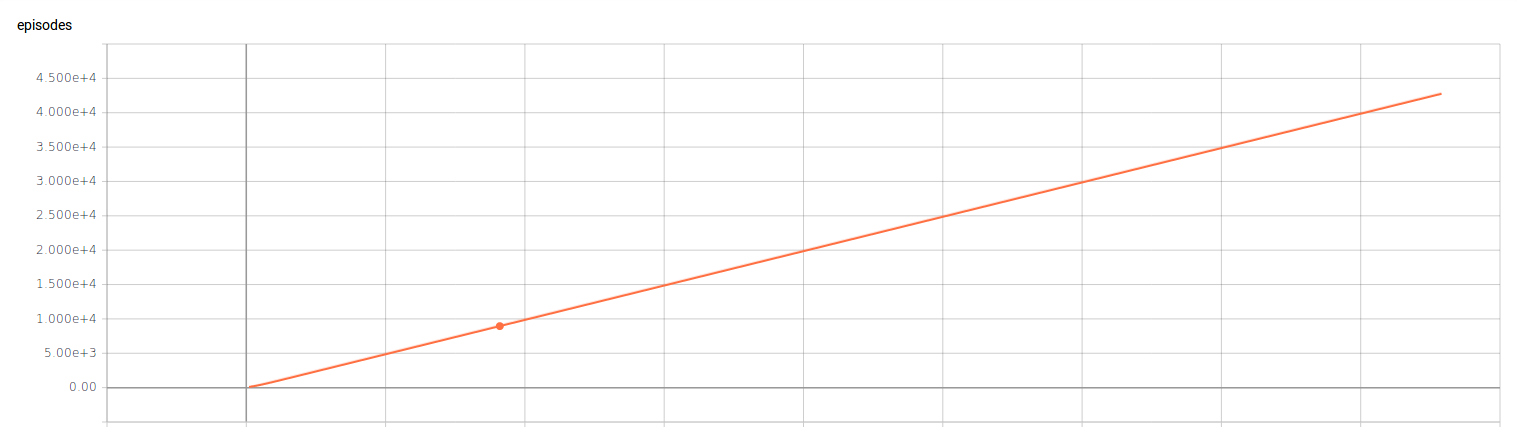
\includegraphics[width=\linewidth]{images/graphs/dqn-episodes-clean.png}
  \caption{DQN Episodes}
  \label{fig:dqn-episodes}
\end{figure}

\begin{figure}[H]
  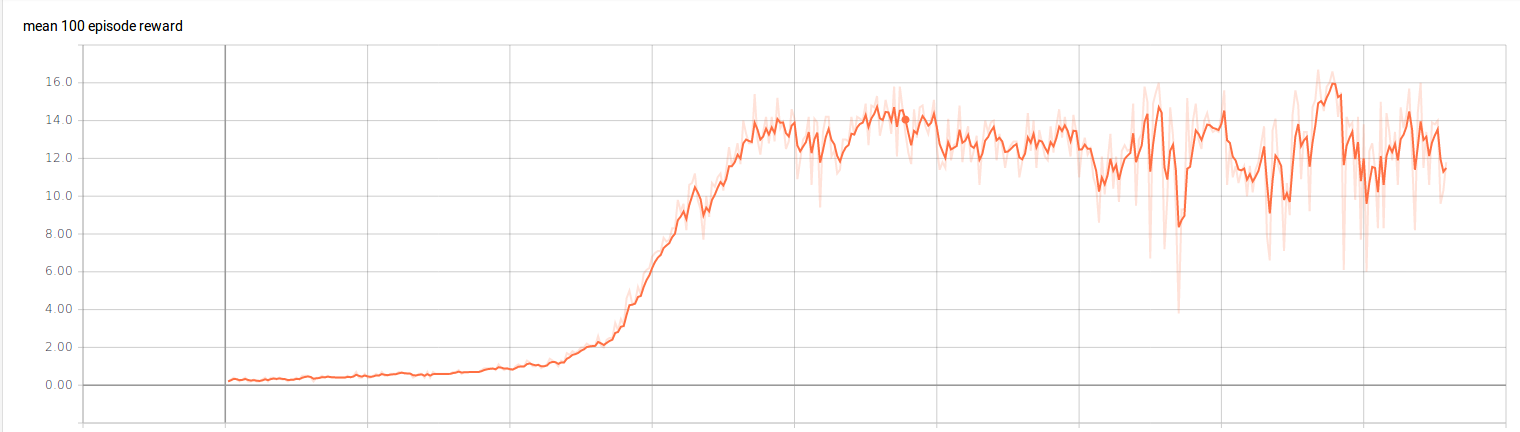
\includegraphics[width=\linewidth]{images/graphs/dqn-mean-100-episode-reward-clean.png}
  \caption{DQN Mean 100 episodes rewards}
  \label{fig:dqn-mean-100-episodes-rewards}
\end{figure}

\begin{figure}[H]
  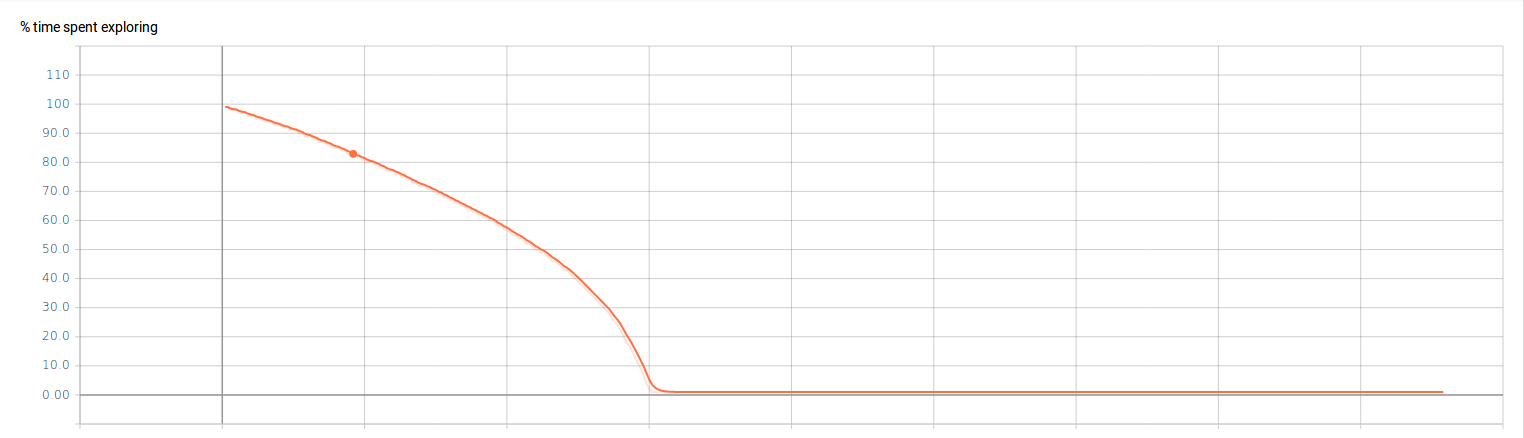
\includegraphics[width=\linewidth]{images/graphs/dqn-percent-time-spent-exploring-clean.png}
  \caption{DQN \% time spent exploring}
  \label{fig:dqn-percent-time-spent-exploring}
\end{figure}

\begin{figure}[H]
  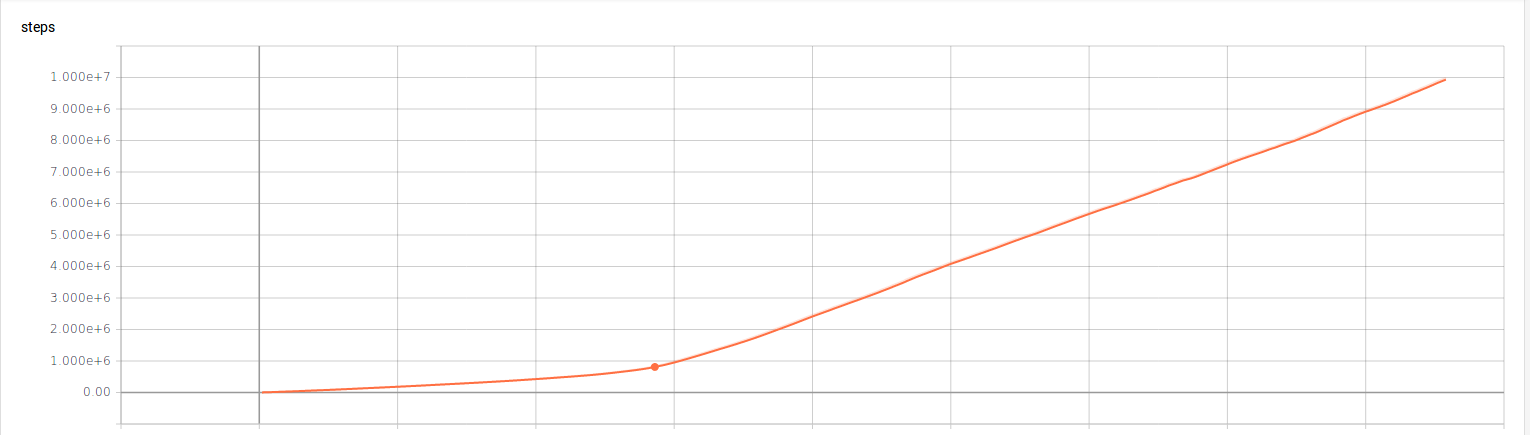
\includegraphics[width=\linewidth]{images/graphs/dqn-steps-clean.png}
  \caption{DQN Steps}
  \label{fig:dqn-steps-clean}
\end{figure}

The graphs indicate the algorithm is improving in playing Breakout. The mean of
100 episode reward increases and it keeps improved after some episodes. In the
beginning, it explores a lot and follows an exploration decay function until it
reaches 0.01 (defined by the parameter \textit{exploration\_final\_eps}).

The problem is what these graphs are not showing. Plotting the graphs with the R
script, we can have more sense in what is really happening.

\begin{figure}[H]
  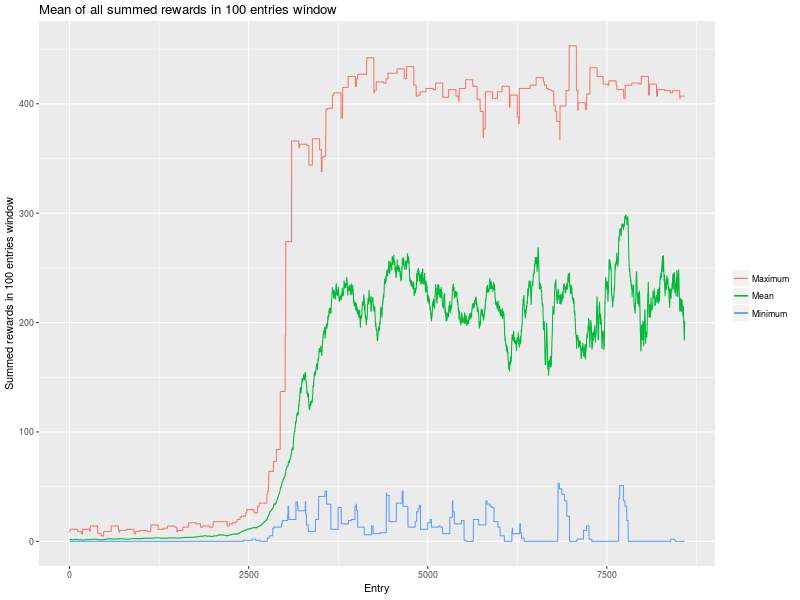
\includegraphics[scale=0.35]{log-analysis/dqn-mean-summed-rewards.png}
  \centering
  \caption{DQN Mean of summed rewards}
  \label{fig:dqn-mean-summed-rewards}
\end{figure}

\begin{figure}[H]
  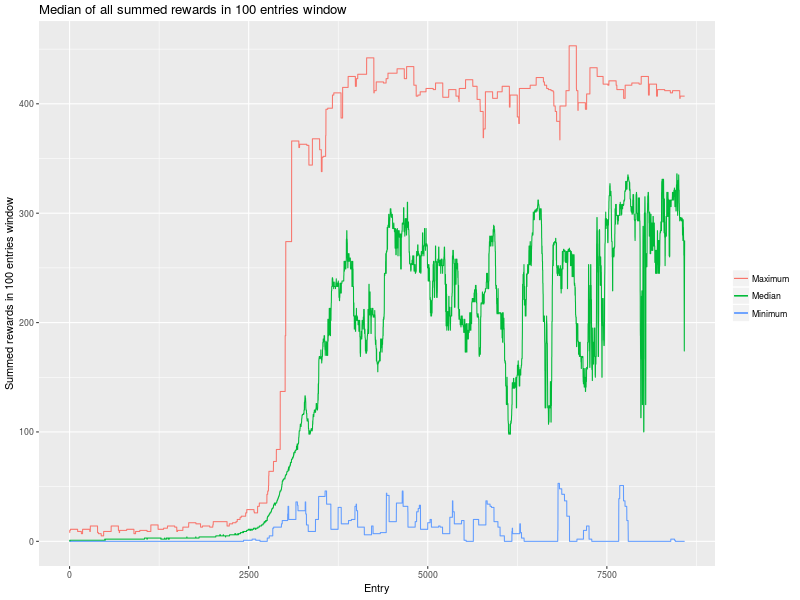
\includegraphics[scale=0.35]{log-analysis/dqn-median-summed-rewards.png}
  \centering
  \caption{DQN Median of summed rewards}
  \label{fig:dqn-median-summed-rewards}
\end{figure}

\begin{figure}[H]
  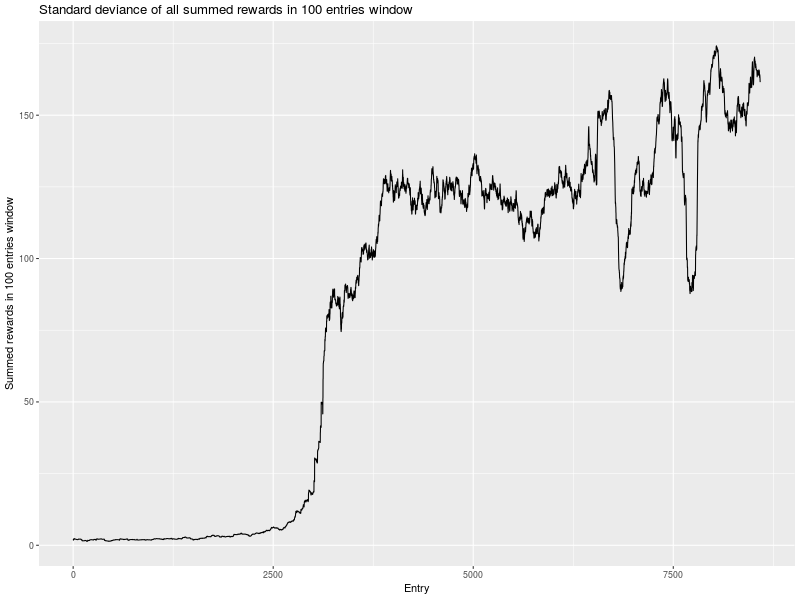
\includegraphics[scale=0.35]{log-analysis/dqn-sd-summed-rewards.png}
  \centering
  \caption{DQN Standard Deviance of summed rewards}
  \label{fig:dqn-sd-summed-rewards}
\end{figure}

It is possible to verify that the improvement in score is not consistent. It
means that sometimes the algorithm really permforms well and in some occasions
the algorithm performs poorly, even much after exploration phase is over. The
median is even more telling in terms of instability.

Checking the number of games played by the algorithm, even more inferences can
be taken:

\begin{figure}[H]
  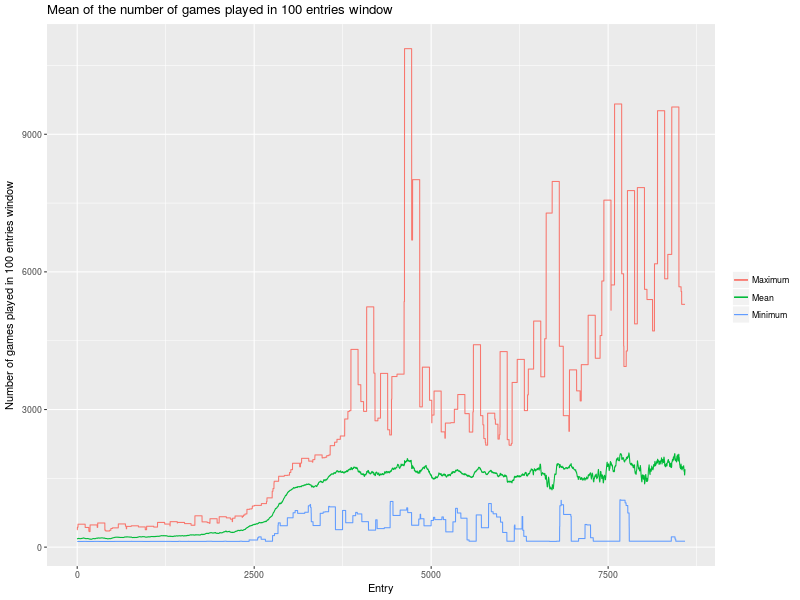
\includegraphics[scale=0.35]{log-analysis/dqn-mean-ngp.png}
  \centering
  \caption{DQN Mean of the number of games played}
  \label{fig:dqn-mean-ngp}
\end{figure}

\begin{figure}[H]
  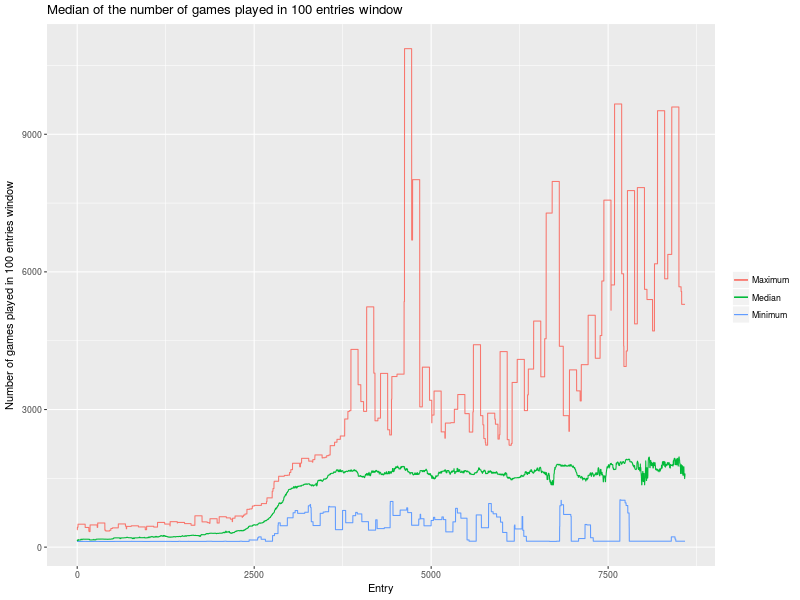
\includegraphics[scale=0.35]{log-analysis/dqn-median-ngp.png}
  \centering
  \caption{DQN Median of the number of games played}
  \label{fig:dqn-median-ngp}
\end{figure}

\begin{figure}[H]
  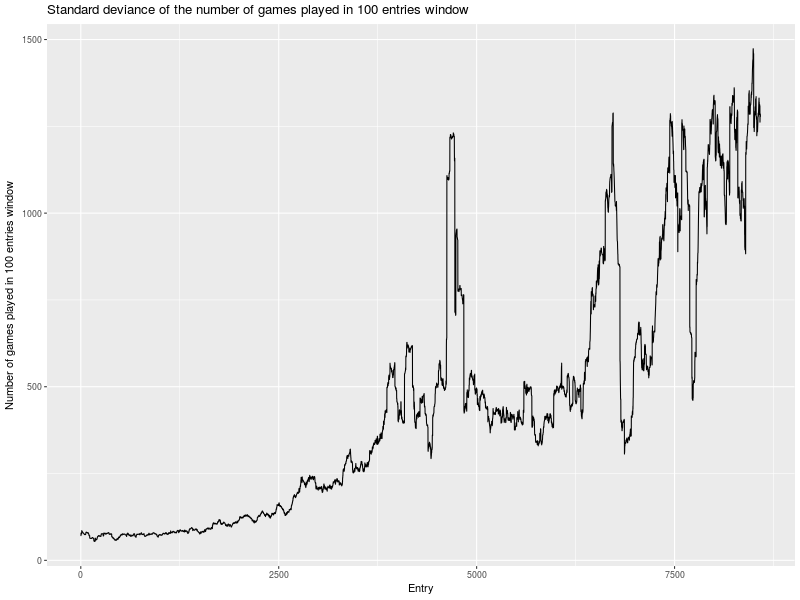
\includegraphics[scale=0.35]{log-analysis/dqn-sd-ngp.png}
  \centering
  \caption{DQN Standard deviation of the number of games played}
  \label{fig:dqn-sd-ngp}
\end{figure}

The graphs reveal that the number of games played varies too much in each episode,
meaning that some good results might have come at the expense of having lots of
games played and summing the score in the sum of scores metric, however it seems
that the DQN improves the scores a little even after, in average, the number of
games played does not increase. Therefore, DQN is, in fact, learning to play
Breakout.

There are some interesting results when the parameter \textbf{dueling} is set
to \textbf{0}.

\begin{figure}[H]
  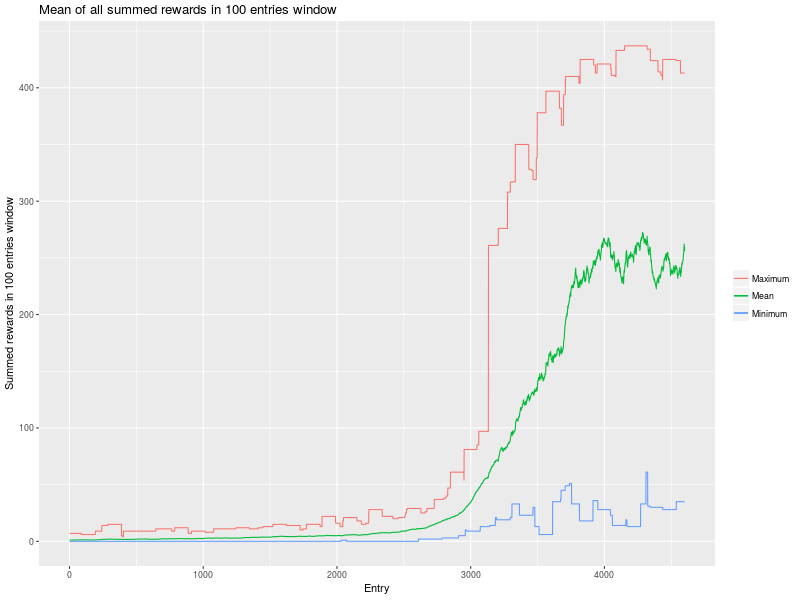
\includegraphics[scale=0.35]{log-analysis/dqn-nd-mean-summed-rewards.png}
  \centering
  \caption{Non-dueling DQN Mean of summed rewards}
  \label{fig:dqn-nd-mean-summed-rewards}
\end{figure}

\begin{figure}[H]
  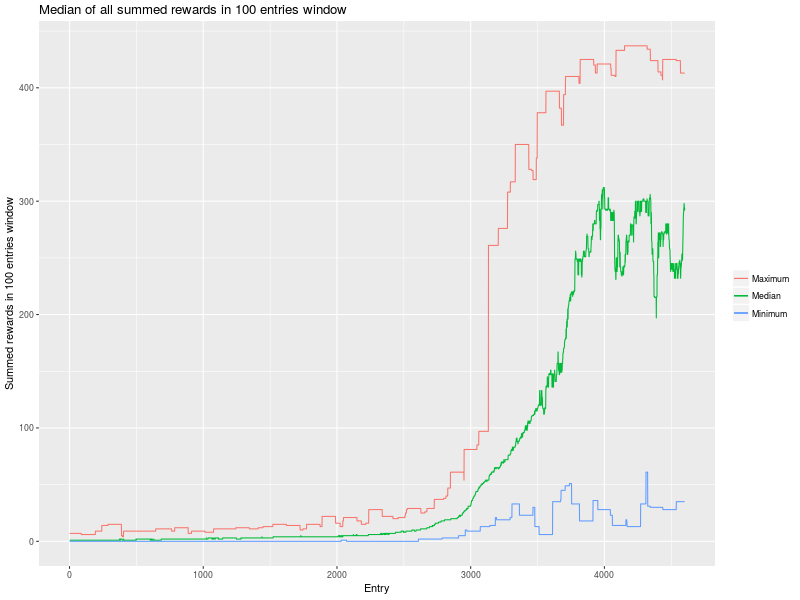
\includegraphics[scale=0.35]{log-analysis/dqn-nd-median-summed-rewards.png}
  \centering
  \caption{Non-dueling DQN Median of summed rewards}
  \label{fig:dqn-nd-median-summed-rewards}
\end{figure}

\begin{figure}[H]
  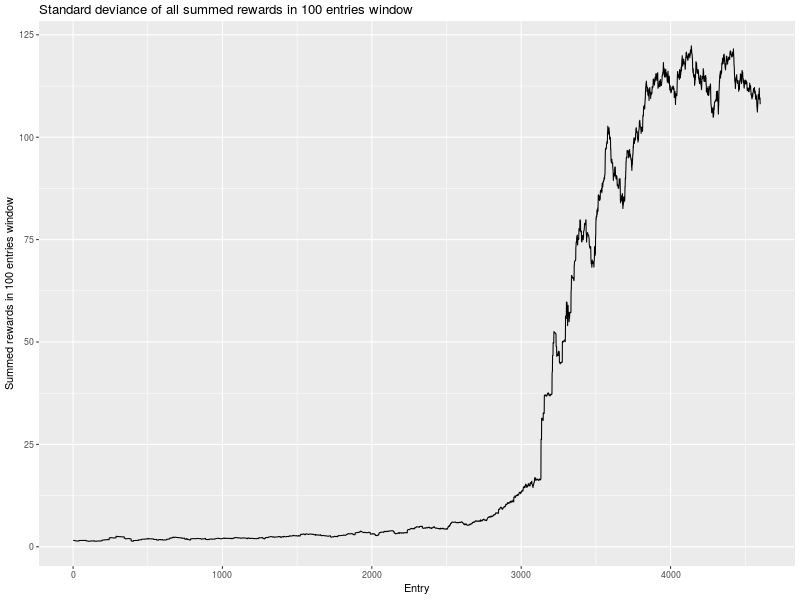
\includegraphics[scale=0.35]{log-analysis/dqn-nd-sd-summed-rewards.png}
  \centering
  \caption{Non-dueling DQN Standard Deviance of summed rewards}
  \label{fig:dqn-nd-sd-summed-rewards}
\end{figure}

\begin{figure}[H]
  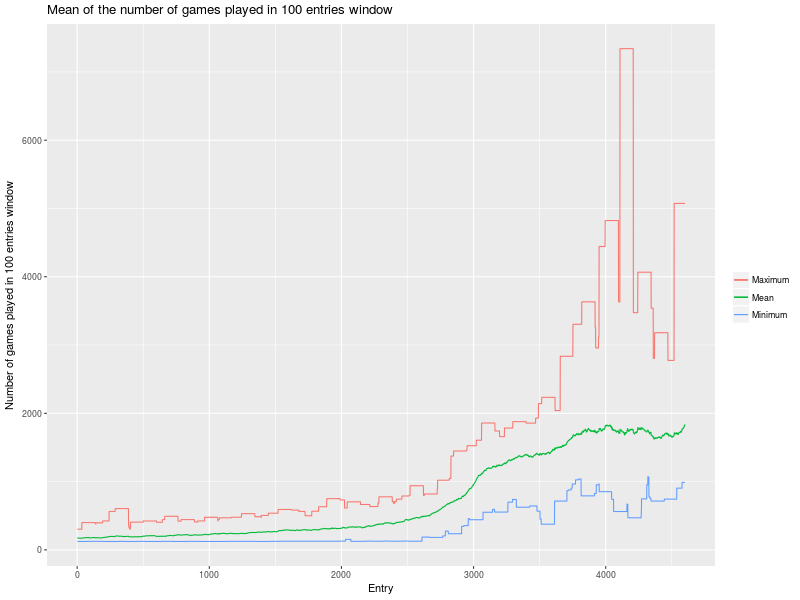
\includegraphics[scale=0.35]{log-analysis/dqn-nd-mean-ngp.png}
  \centering
  \caption{Non-dueling DQN Mean of the number of games played}
  \label{fig:dqn-nd-mean-ngp}
\end{figure}

\begin{figure}[H]
  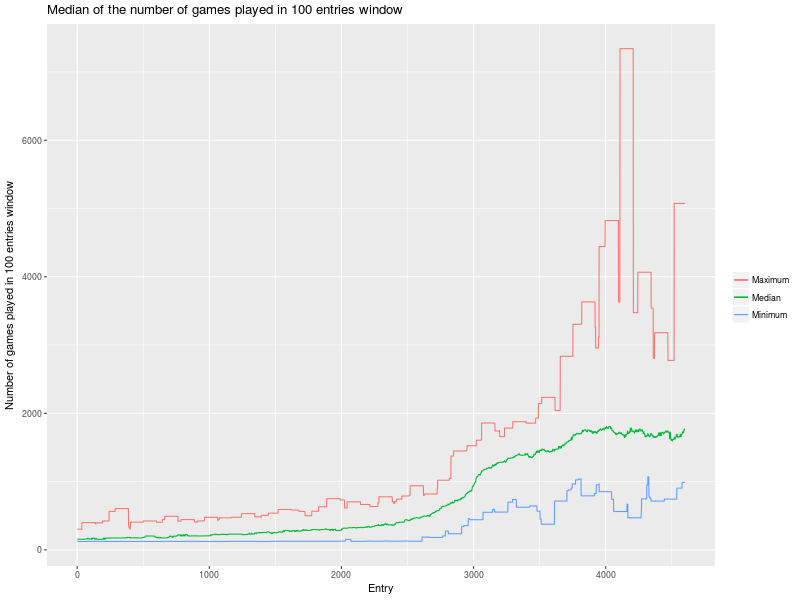
\includegraphics[scale=0.35]{log-analysis/dqn-nd-median-ngp.png}
  \centering
  \caption{Non-dueling DQN Median of the number of games played}
  \label{fig:dqn-nd-median-ngp}
\end{figure}

\begin{figure}[H]
  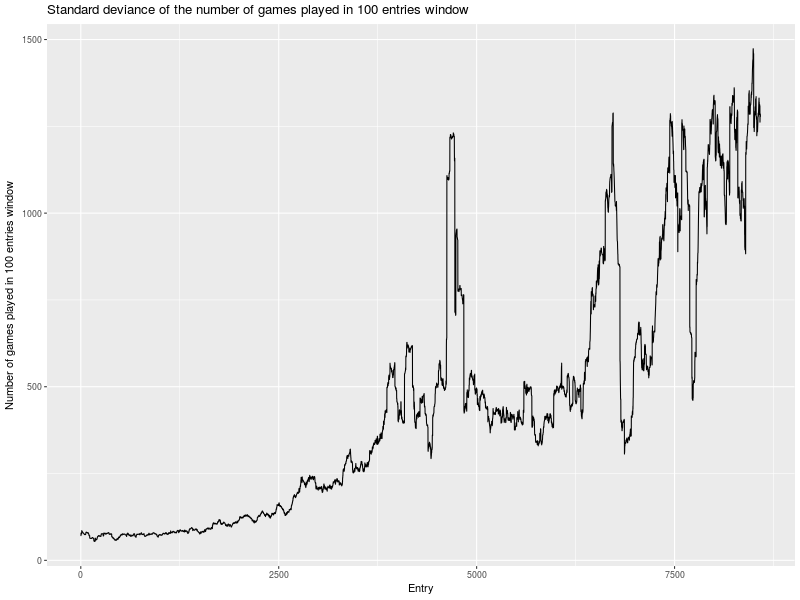
\includegraphics[scale=0.35]{log-analysis/dqn-nd-sd-ngp.png}
  \centering
  \caption{Non-dueling DQN Standard deviation of the number of games played}
  \label{fig:dqn-nd-sd-ngp}
\end{figure}

The training time increases to 24 hours (for this amount of time, the precision
of minutes becomes irrelevant). In addition, it take less entries to converge,
however the entries takes longer to finish. It seems the learning is more
stable, steady, and its results are 7\% to 58\% better in terms of final score.
It is slower and converges to the best value Dueling-DQN obtained in around 7
hours, though.

\subsection*{A2C}

Some of these graphs are more challenging to read for non-academics and to
associate the information the bring to what is happening to the agent. Let us
delve into them.

\begin{figure}[H]
  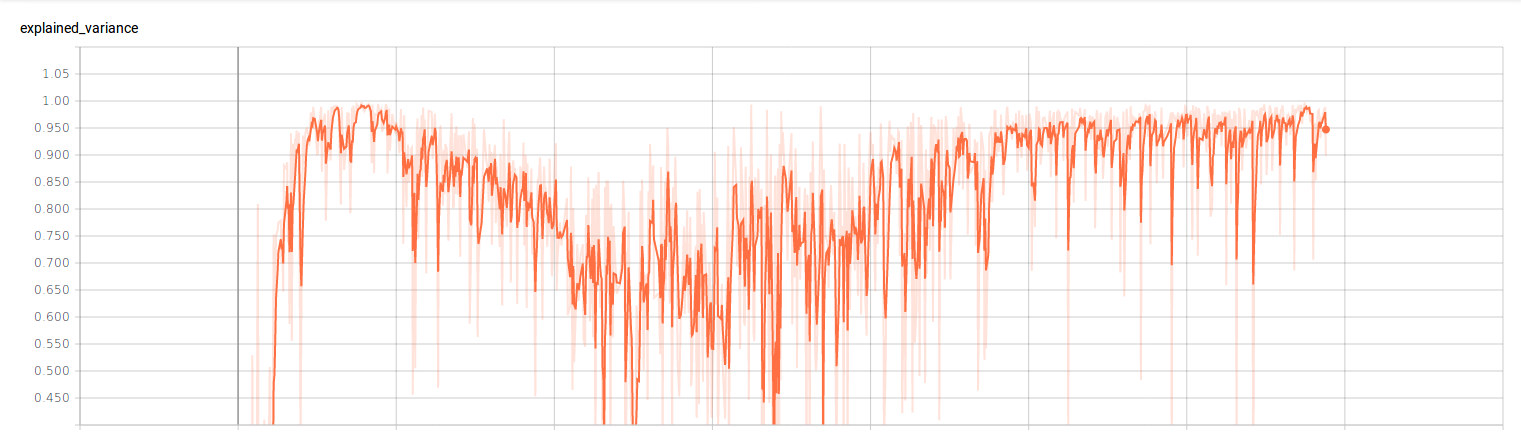
\includegraphics[scale=0.30]{images/graphs/a2c-explained_variance-clean.png}
  \centering
  \caption{A2C Explained Variance}
  \label{fig:a2c-explained_variance}
\end{figure}

Here we can see that the explained variance starts close to 1, decreases, and
goes back to be close to 1. The explained variance is how much the predicted
\emph{y} value explains about \emph{y}. The formula for the explained variance
is:

$$
1 - \frac{Var[y-ypred]}{Var[y]}
$$

\begin{figure}[H]
  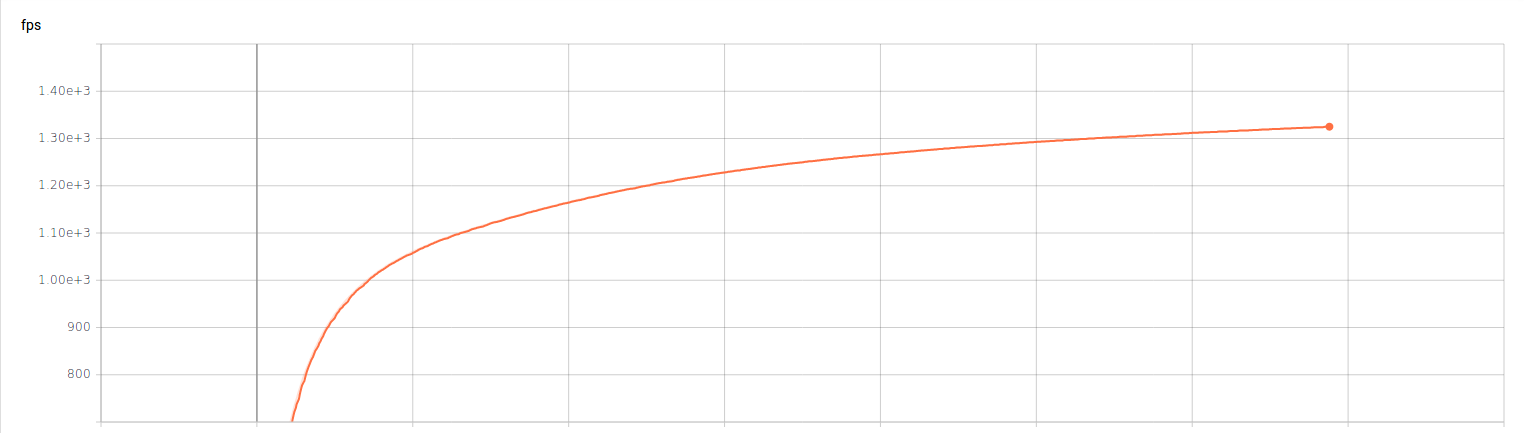
\includegraphics[scale=0.30]{images/graphs/a2c-fps-clean.png}
  \centering
  \caption{A2C FPS}
  \label{fig:a2c-fps}
\end{figure}

\begin{figure}[H]
  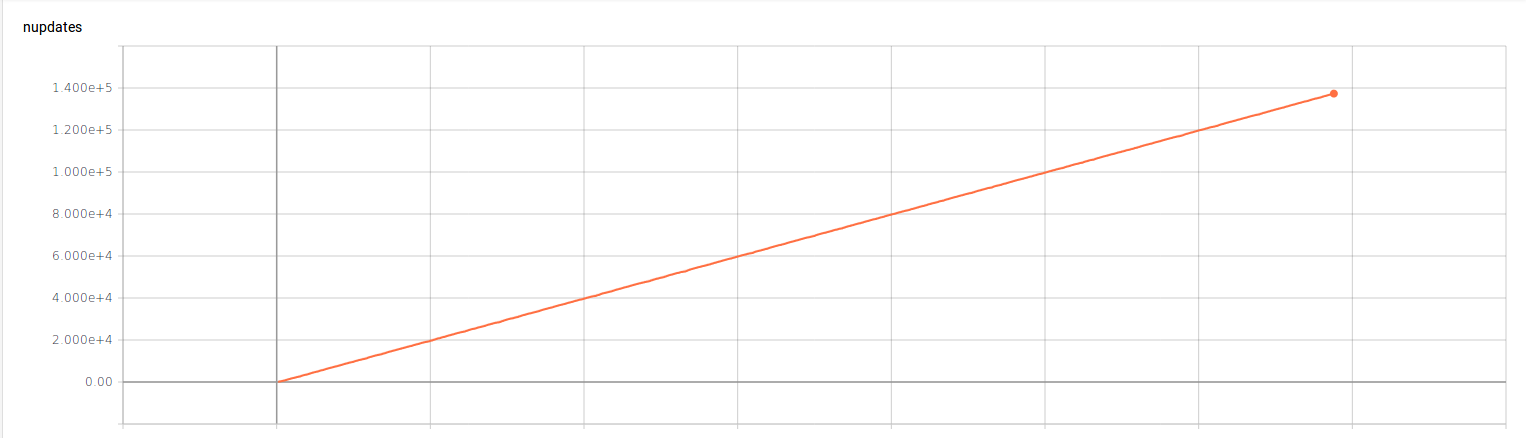
\includegraphics[scale=0.30]{images/graphs/a2c-nupdates-clean.png}
  \centering
  \caption{A2C Number of updates}
  \label{fig:a2c-nupdates}
\end{figure}

\begin{figure}[H]
  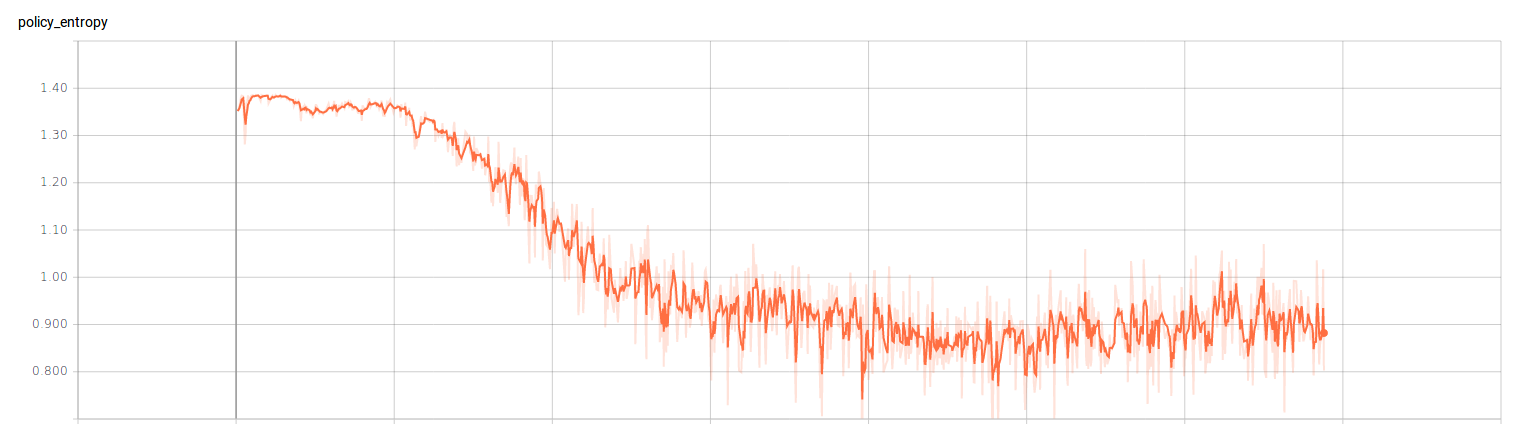
\includegraphics[scale=0.30]{images/graphs/a2c-policy-entropy-clean.png}
  \centering
  \caption{A2C Policy entropy}
  \label{fig:a2c-policy-entropy}
\end{figure}

Policy entropy is technique to discourage the premature convergence of the
policy by adding some entropy and force the agent to explore more, instead to
converge to a suboptimal policy, as described in A3C per-print
\cite{DBLP:journals/corr/MnihBMGLHSK16}. The function that executes this
calculation is \textit{cat\_entropy} and it is in
\textit{baselines/a2c/utils.py}.

The graph points out that the entropy reduces to a value below 1 and oscilate
around 0.9, indicating that the agent is still encourage to explore, even if it
is converging, which seems to be doing so.

\begin{figure}[H]
  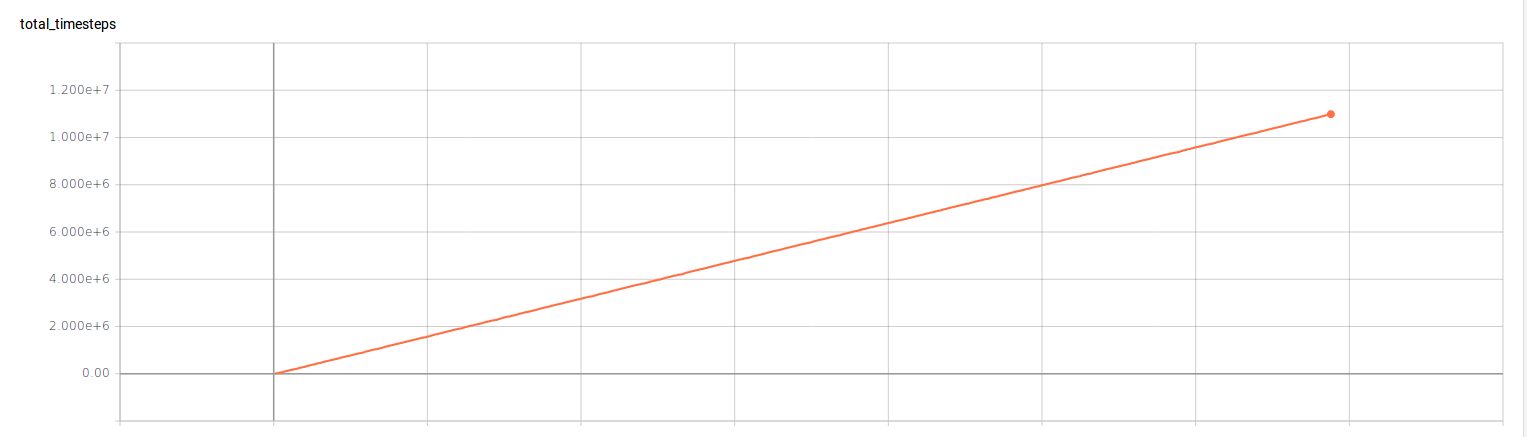
\includegraphics[scale=0.30]{images/graphs/a2c-total-timesteps-clean.png}
  \centering
  \caption{A2C Total timesteps}
  \label{fig:a2c-total-timesteps}
\end{figure}

\begin{figure}[H]
  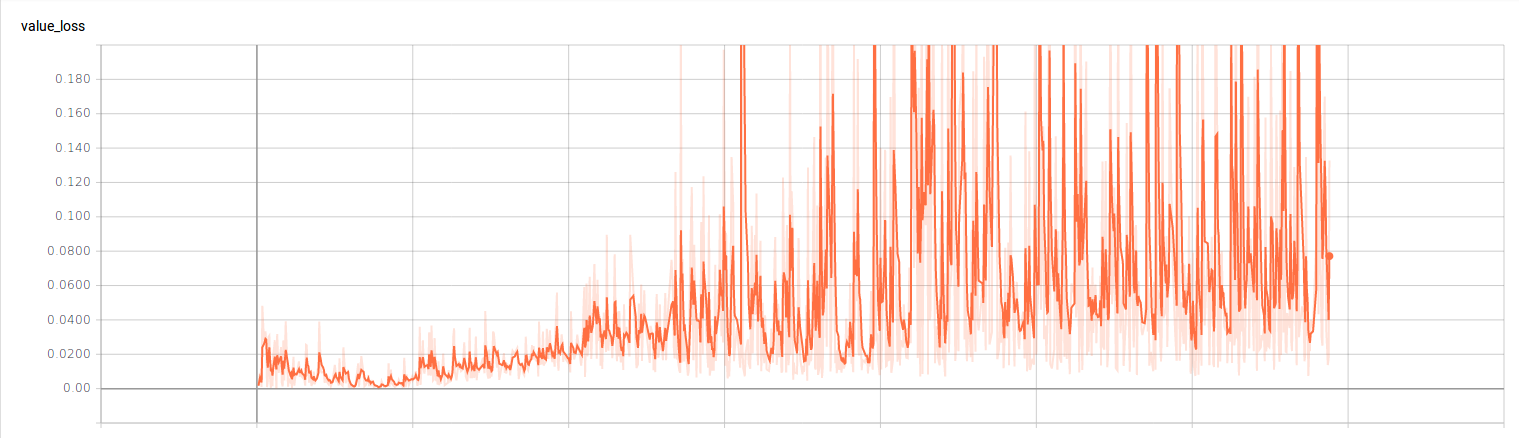
\includegraphics[scale=0.30]{images/graphs/a2c-value-loss-clean.png}
  \centering
  \caption{A2C Value Loss}
  \label{fig:a2c-value-loss-clean}
\end{figure}

Now, let us visualize the graphs obtained from CSV data.

\begin{figure}[H]
  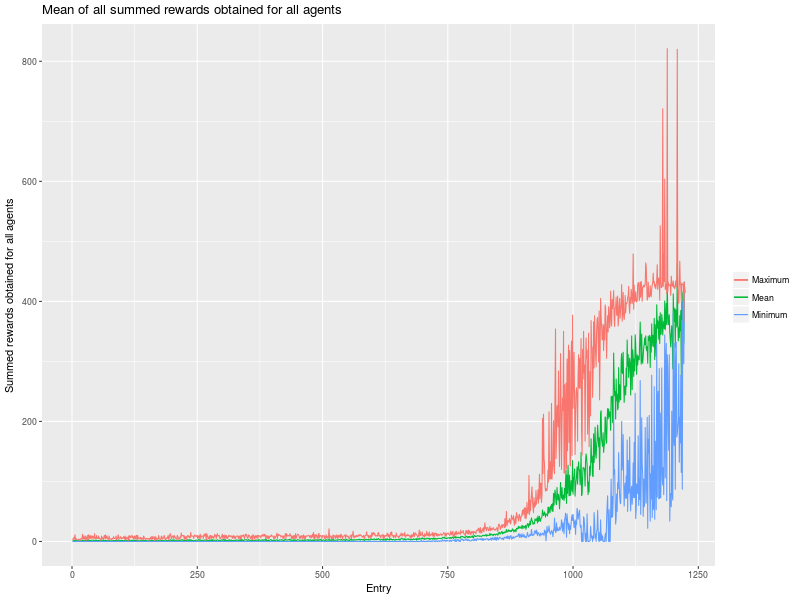
\includegraphics[scale=0.35]{log-analysis/a2c-mean-summed-rewards.png}
  \centering
  \caption{A2C Mean of summed rewards}
  \label{fig:a2c-mean-summed-rewards}
\end{figure}

\begin{figure}[H]
  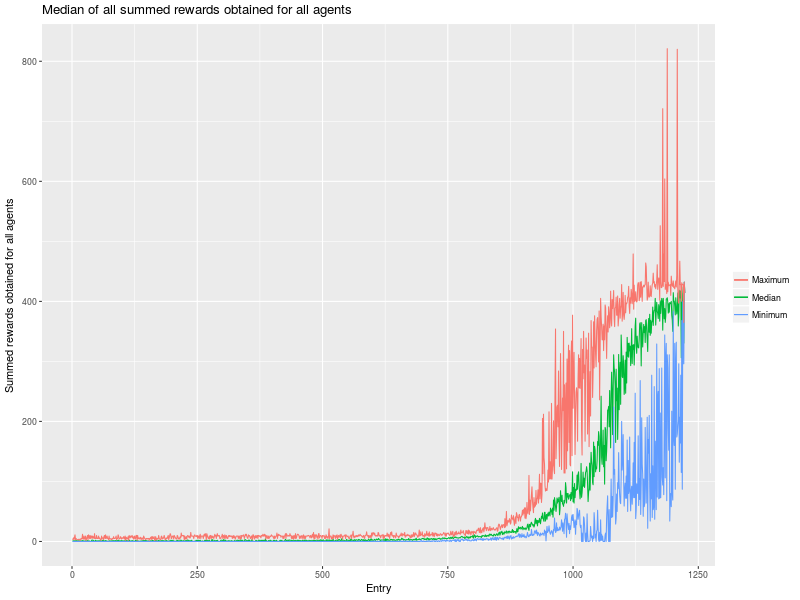
\includegraphics[scale=0.35]{log-analysis/a2c-median-summed-rewards.png}
  \centering
  \caption{A2C Median of summed rewards}
  \label{fig:a2c-median-summed-rewards}
\end{figure}

\begin{figure}[H]
  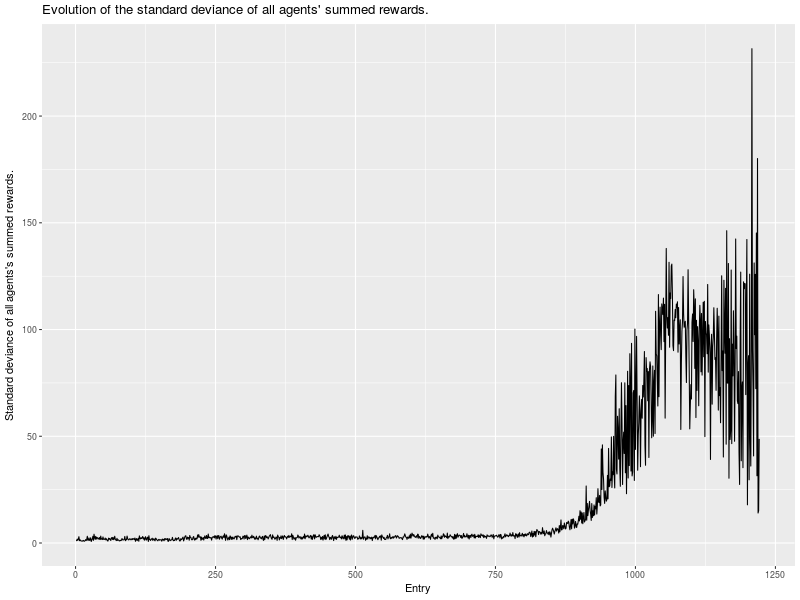
\includegraphics[scale=0.35]{log-analysis/a2c-sd-summed-rewards.png}
  \centering
  \caption{A2C Standard Deviance of summed rewards}
  \label{fig:a2c-sd-summed-rewards}
\end{figure}

Even though the graphs seems to indicate more instability, this is an effect of
having merged information from 16 learners and not having smoothed between N
episodes. Despite that, it seems that this algorithm obtain better scores,
converges to an optimal policy, and its standard deviance of all agent's summed
reward appears to be trending to less than 100 (in Breakout score metric).

\begin{figure}[H]
  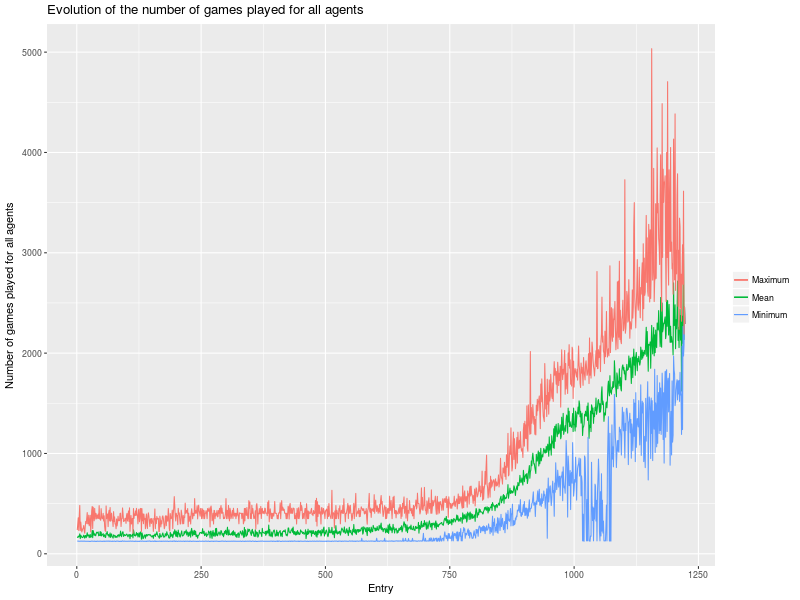
\includegraphics[scale=0.35]{log-analysis/a2c-mean-ngp.png}
  \centering
  \caption{A2C Mean of the number of games played}
  \label{fig:a2c-mean-ngp}
\end{figure}

\begin{figure}[H]
  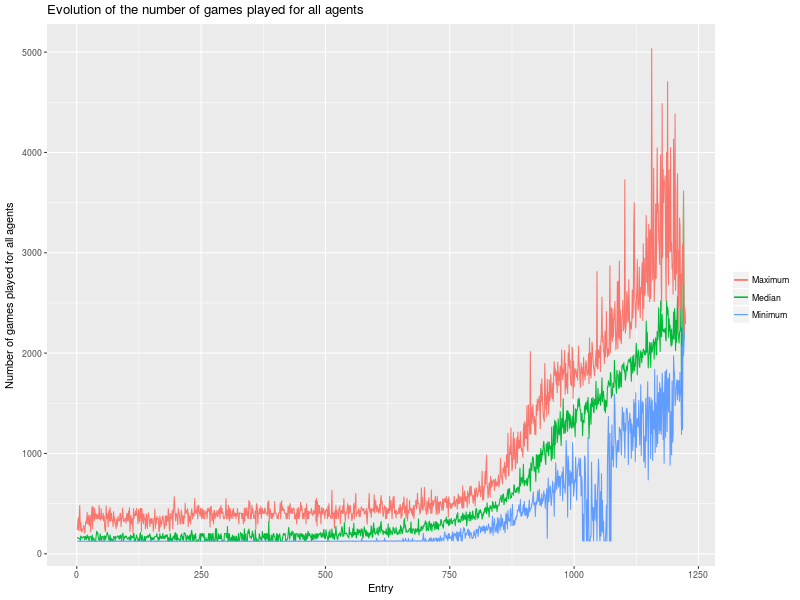
\includegraphics[scale=0.35]{log-analysis/a2c-median-ngp.png}
  \centering
  \caption{A2C Median of the number of games played}
  \label{fig:a2c-median-ngp}
\end{figure}

\begin{figure}[H]
  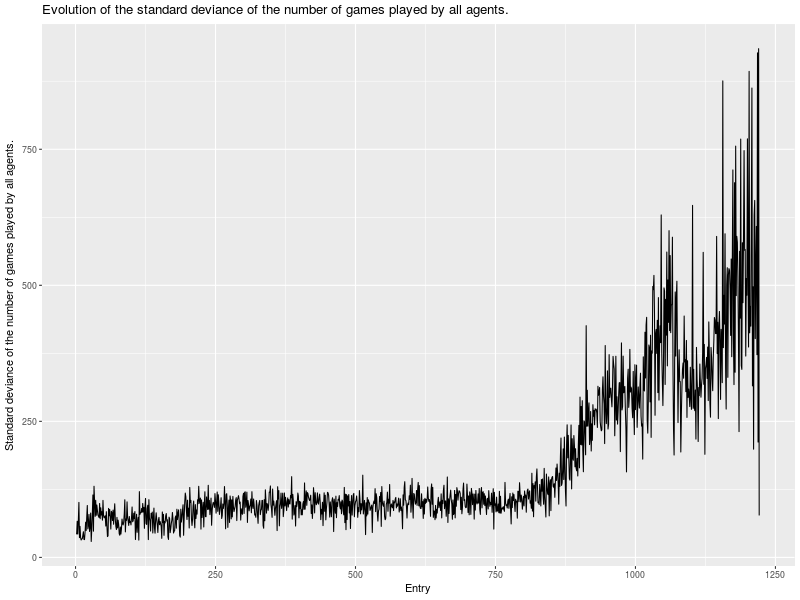
\includegraphics[scale=0.35]{log-analysis/a2c-sd-ngp.png}
  \centering
  \caption{A2C Standard deviation of the number of games played}
  \label{fig:a2c-sd-ngp}
\end{figure}

Examining the graphs of the number of games played from A2C agent (or agents),
it reveals that the number of games played is higher, from around 1500 from DQN
to around 2000 from A2C. In spite of playing more games, the standard deviance
of the number of games played is close to a half of DQN's standard deviance in
the number of games played. This algorithm seems more consistent in this aspect.

\subsection*{Comparison between all experiments}

From the experiments done, we can compare the execution times, mean summed score,
median summed score, standard deviance of the summed score. From this comparison,
A2C with CNN policy and constant learning rate schedule reveals to be the best
algorithm and parameters evaluanted.

In the table below, I condensed the running time of the algorithm and last
entries for mean, median, and standard deviance reported by the algorithm. A2C,
by its nature of multiple agents, end up finishing its execution with one agent.
Therefore, no entry for standard deviance will be reported.

\begin{center}
  \begin{tabular}{ | l | c | c | c | r | }
    \hline
    \textbf{Algorithm} & \textbf{Time} & \textbf{Mean} & \textbf{Median} & $ \boldsymbol{\sigma} $ \\ \hline
    DQN 1st run, dueling & 21h 16min & 201.6471  & 275.0 & 161.5241 \\ \hline
    DQN 2nd run, dueling & 20h 36min & 185.2157 & 186.0  & 117.0529 \\ \hline
    DQN, non-dueling & 1d 0h 16min & 259.4902 & 294.0 & 108.0432 \\ \hline
    A2C 1st run, cnn, constant & 2h 14min & 414.0 & 414.0 & - \\ \hline
    A2C 2nd run, cnn, constant & 2h 7min & 368.0 & 368.0 & - \\ \hline
    A2C, cnn, linear & 2h 8min & 356.0 & 356.0 & - \\ \hline
    A2C, lstm, constant & 2h 19min & 387.0 & 387.0 & - \\ \hline
    A2C, lstm, linear & 2h 19min & 93.0 & 93.0 & - \\ \hline
    A2C, lnlstm, constant & 2h 31min & 417.0 & 417.0 & - \\ \hline
    A2C, lnlstm, linear & 2h 37min & 160.0 & 160.0 & - \\
    \hline
  \end{tabular}
\end{center}

It is curious how learning rate schedule influentiates in the performance of A2C
algorithm, even more in LSTM and LNLSTM policies. Constant learning rate
schedule are the best one for this algorith. The change in the neural network
architecture seems to be not influentiate much in the performance of the learner.

Examining the LNLSTM case:

\begin{figure}[H]
  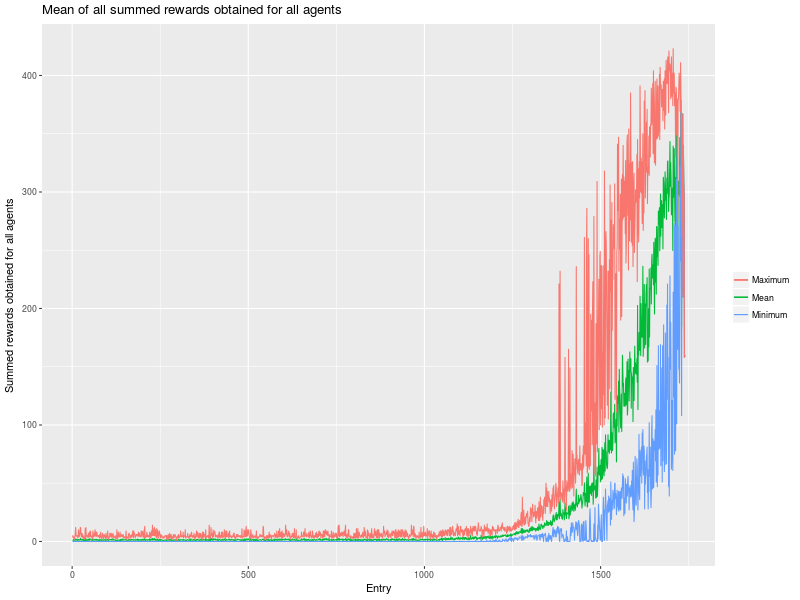
\includegraphics[scale=0.35]{log-analysis/a2c-lnlstm-mean-summed-rewards.png}
  \centering
  \caption{A2C LNLSTM Mean of summed rewards}
  \label{fig:a2c-lnlstm-mean-summed-rewards}
\end{figure}

we see that there are not spikes and it looks like to be less variant than the
A2C that uses CNN as policy neural network. From the graphs above, the choice
for A2C with all standard parameters seem to be a reasonable choice to be the
final model.

\section*{Conclusion}

Examining both DQN and A2C, I conclude that DQN requires too much compute time
to converge and It achieves good results. A2C achieve better results in a
fraction of DQN's compute time. It might be too expensive in terms of compute
resources to reproduce studies that uses DQN because it requires GPU and lots of
time to converge, if it converges. On the other hand, A2C does not require GPUs
and requires less resources to run, saving user's money and time.

However, one question remained unaswered: does this model beats the average of
the 10 best humans in Breakout? The baseline is a mean of 580.9 and a median of
494. Comparing with the results of A2C:

\begin{figure}[H]
  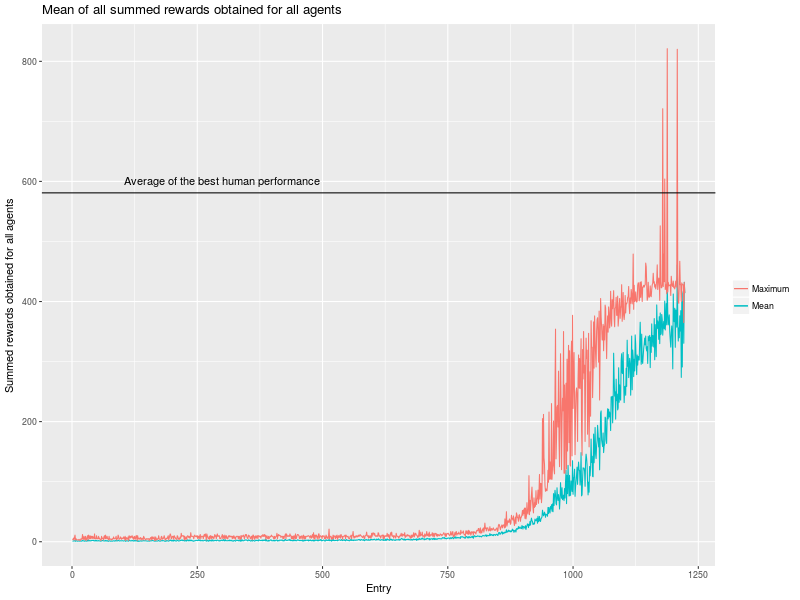
\includegraphics[scale=0.35]{log-analysis/a2c-vs-humans-mean.png}
  \centering
  \caption{A2C mean of summed rewards vs humans}
  \label{fig:a2c-vs-humans-mean}
\end{figure}

\begin{figure}[H]
  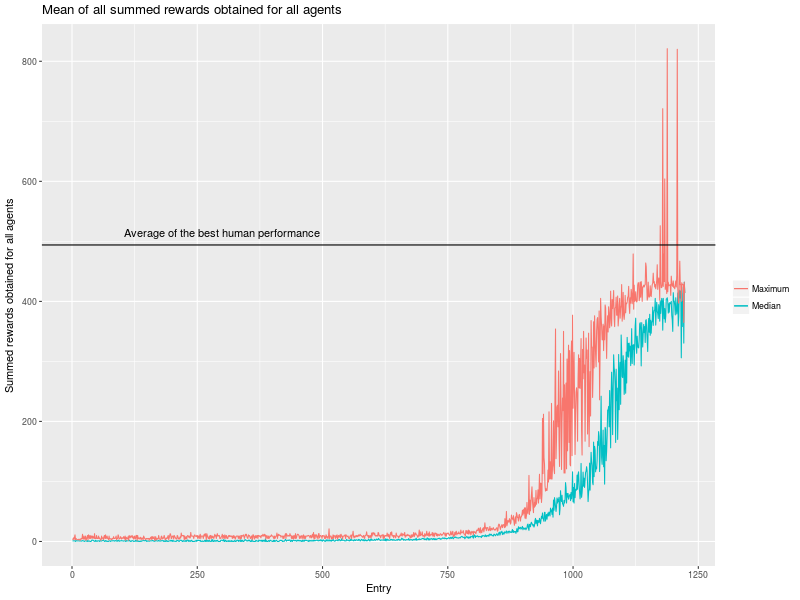
\includegraphics[scale=0.35]{log-analysis/a2c-vs-humans-median.png}
  \centering
  \caption{A2C median of summed rewards vs humans}
  \label{fig:a2c-vs-humans-median}
\end{figure}

From the graphics above, we can conclude that Deep Reinforcement Learning is
close to the best human performance, but it is wrong conclusion, since it is a
summed reward versus a single best reward. What we can conclude is that the
algorithms are able to learn to play Breakout and, trying hard, achieve human
level scores.

\subsubsection*{Reflections}

In this project I used the following process:

\begin{enumerate}
  \item Preparate the OpenAI baselines code to setup the log formats in the
  start of the script.
  \item Manually composed an AMI, based on Deep Learning AMI 2.0 from AWS.
  \item Create a shell and execute the algorithms from my choice.
  \item Extracted the results.
  \item Read the references from Arxiv and Nature.
  \item Wrote a summary for each algorithm.
  \item Composed graphs and analyzed the results.
\end{enumerate}

The interesing parts of the project were analyze OpenAI baselines code and
fiddle with it and execute it in an AWS EC2 instance (this was also expensive).
The challenging parts were reading all the papers, extract the most essential
items from them, understand the math and where it was in the code. Implement
math in TensorFlow is challenging, but not difficult.

Since I was expecting nothing but understand the DRL algorithms, I am initially
happy with the results attained. Of course I want to improve over them, but it
is a matter of time. However, I would not use DQN to solve any DRL problem,
except if any other DQL algorithm have inadequate performance. A3C and A2C
should be used as baselines, in my opinion.

\subsubsection*{Improvements}

This project could be improved if I had more math knowledge and more time and
money to invest in a more ambitios endeavor. I would try to compare A2C with
ACKTR and ACER (links in the next section). The algorithms I used are totally
refined, so no further improvements could be done.

The Deep Reinforcement Learning field is in its infancy. Any pre-print newer
than the articles I have used for this capstone might have better results. Thus,
the dedication to learn advanced math and examine complex publications are
fundamental to succeed into improve this capstone project.

\subsubsection*{Future studies}

For the future, I want to study:

\begin{itemize}
  \item Multivariate Calculus
  \item Differential Equations
  \item Stochastic processes
\end{itemize}

in order to understand research made by OpenAI and DeepMind. I intend to read
carefully the pre-prints \url{https://arxiv.org/abs/1611.01224} and
\url{https://arxiv.org/abs/1708.05144}. There are newer pre-prints to read and
to try, such as DeepMind IMPALA, in \url{https://arxiv.org/abs/1802.01561}.

I am also going try to implement these algorithms myself, using the material in
\url{https://sites.google.com/view/deep-rl-bootcamp/labs} and add all
improvements learnt during the work in this capstone project.

\bibliographystyle{plain}
\bibliography{bibliography}

\end{document}
